\chapter{Atmospheric muons and the LUX-ZEPLIN experiment}\label{chap:Muons}
Atmospheric muons pose a threat through direct detection dark matter searches such as LZ. Energetic neutrons which could mimic a dark matter signal can be produced through muon interactions with detector and the surrounding materials \cite{LZ_SIMS}. To decrease the impact that atmospheric muons have on rare event searches, experiments are situated at deep underground sites. 
The production mechanisms for atmospheric muons from cosmic ray and how the intensity of the muon flux varies between the Earth's surface and at underground sites is first discussed in \autoref{sec:Muons/CosmicRays} and \autoref{sec:Muons/MuonsUnderground}. How muons interact as they travel through materials and induced backgrounds from such interactions is discussed in \autoref{sec:Muons/MuonTransport} and \autoref{sec:Muons/InducedBackgrounds}. The measurement of the muon flux through the LZ experiement is presented in \autoref{sec:Muons/MuonFluxMeasurementWithLZ} alongside the impact that muons have on the WIMP and the measures taken to veto muons events and the aftermath left in the detector after a muon has travelled through, discussed in \autoref{sec:Muons/MuonVeto}. How the muon flux in LZ modulates over time is discussed in \autoref{sec:Muons/MuonModulation}.

\section{Cosmic rays and atmospheric muons}\label{sec:Muons/CosmicRays}
Atmospheric showers are produced from the collision of primary cosmic radiation with the upper Earth's atmosphere. Primary cosmic radiation can be attributed to a non-thermal population of particles that pervade the Universe \cite{ParticleDataGroup:2024cfk}. The charged cosmic rays (CRs) consist mostly of nuclei and electrons at a ratio of 49:1, where the majority of the nuclei are Hydrogen (87\%) and Helium (12\%) with 1\% in the form of heavier elements \cite{Longair_2011}. The energy spectrum of primary CRs can be described using the following power law:
\begin{equation}\label{eqn:CREnergy}
    \frac{E^2dJ}{dE}\sim E^{-\gamma},
\end{equation}
where the spectral index, $\gamma$, varies across the energy spectrum in the range of $2.5\lesssim\gamma\lesssim3$ \cite{ParticleDataGroup:2024cfk}. Charged CRs follow a power law with a spectral index $\gamma\simeq2.7$ for energies up to a few PeV. The combined energy spectra for charged CRs, gamma-rays and neutrinos is shown in \autoref{fig:Muons/CREnergySpec}.
\begin{figure}[ht!]
    \centering
    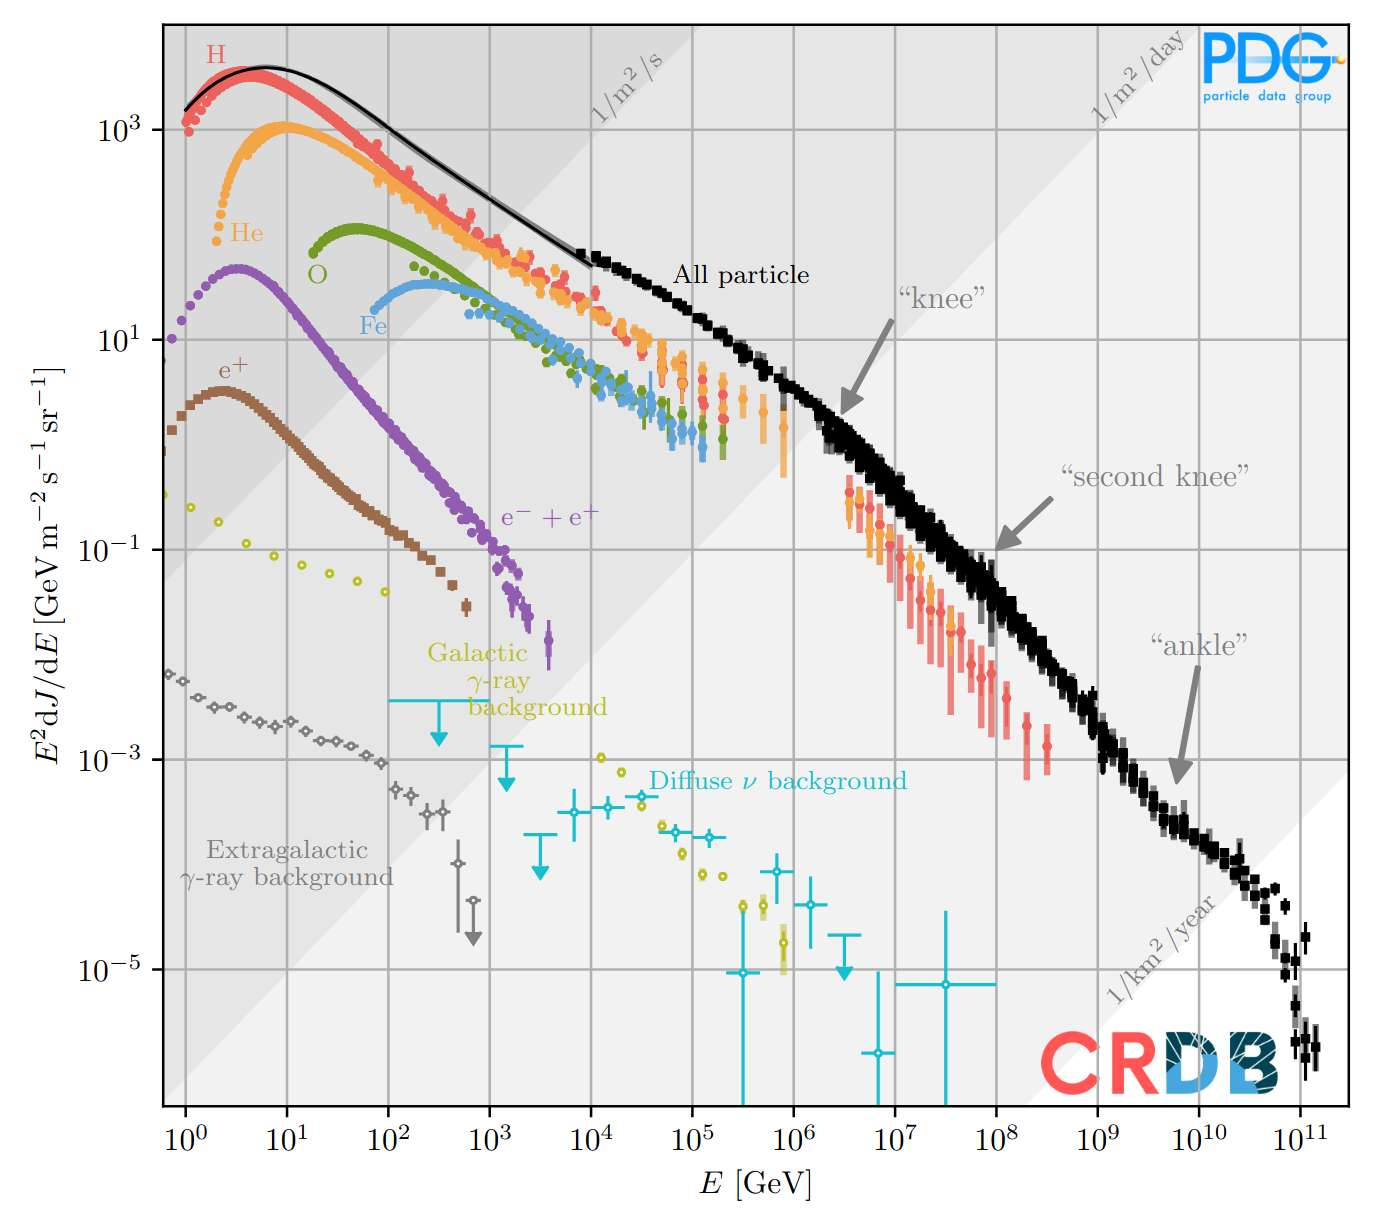
\includegraphics[width=0.7\linewidth]{figures/Muons/CosmicRaySpectra.png}
    \caption{The spectrum of cosmic rays (CRs), diffuse gamma-rays and neutrinos. The measurements of intensity of charged and neutral CRs multiplied by the kinetic energy squared. Energy-integrated intensities are shown by the various diagonal lines. Figure reprinted from Ref.\cite{ParticleDataGroup:2024cfk}.}
    \label{fig:Muons/CREnergySpec}
\end{figure}
A number of secondary particles are produced through CR interactions with atmospheric nuclei. For high energy protons ($\geq 1~\text{GeV}$), the de Broglie wavelength of the incident particle is much less than the distance between nucleons in the nucleus \cite{Longair_2011}. Therefore we can consider the proton as being very discrete and will interact with individual nucleons within the nucleus. In the collision, pions of all charges, $\pi^+,\:\pi^-\text{, and }\pi^0$ are the principle products. In additions to these mesons, the nucleons involved in the interaction may also be expelled from the nucleus. This results in the nucleus being left in a highly unstable excited state that ejects several nuclear fragments in the form of other light nuclei, protons and/or neutrons. These are called spallation fragments. Further reactions in the form of nucleonic cascades are induced by these products, as well as pions, kaons and other mesons.

Nucleons and charged pions with sufficient energy will continue to multiply in successive collisions until the energy per particle drops below the threshold required for multiple pion productions, also known as \textit{pionisation} \cite{Longair_2011}. Pions have very short lifetimes and decay. Neutral pions decay to two $\gamma$-rays ($\pi^0\rightarrow2\gamma$), which initiate electromagnetic cascades through the conversion into an electron-positron pair ($\gamma\rightarrow e^-+e^+$). The electromagnetic shower is formed through the continued succession of pair production and bremsstrahlung processes. Charged pions decay into muons through the following reactions:
\begin{equation}
\begin{split}
    \pi^+&\rightarrow\mu^++\nu_\mu \\
    \pi^-&\rightarrow\mu^-+\bar\nu_\mu
\end{split}
\end{equation}
Other mesons, such as kaons, have analogous decay processes. Very high energy muons are produced in the uppermost layers of atmosphere before the pions make further nuclear interaction. Muons have virtually no nuclear interactions and are very penetrating. In the rest frame of the muon, they decay with a mean lifetime of $2.2\times10^{-6}~\text{s}$. However, to an external observer they decay with an observed lifetime of $2.2\times10^{-6}\gamma~\text{s}$ due to relativistic time dilation where $\gamma$ is the Lorentz factor. At high energies, the incoming muons have Lorentz factors $\gamma\geq20$ resulting in a time dilation and length contraction which enables them to reach the Earth's surface. 

Lower energy muons have time to decay in-flight into electrons, positrons, and neutrinos that can go on to produce further low-energy electromagnetic showers:
\begin{equation}
\begin{split}    
    \mu^+&\rightarrow e^++\nu_e+\bar\nu_\mu \\
    \mu^-&\rightarrow e^-+\bar\nu_e+\nu_\mu
\end{split}
\end{equation}
The interaction of a primary cosmic ray in the atmosphere and the subsequent interactions of the products from the nucleonic cascades are depicted in a diagram shown in \autoref{fig:Muons/CRDiagram}.
\begin{figure}[ht!]
    \centering
    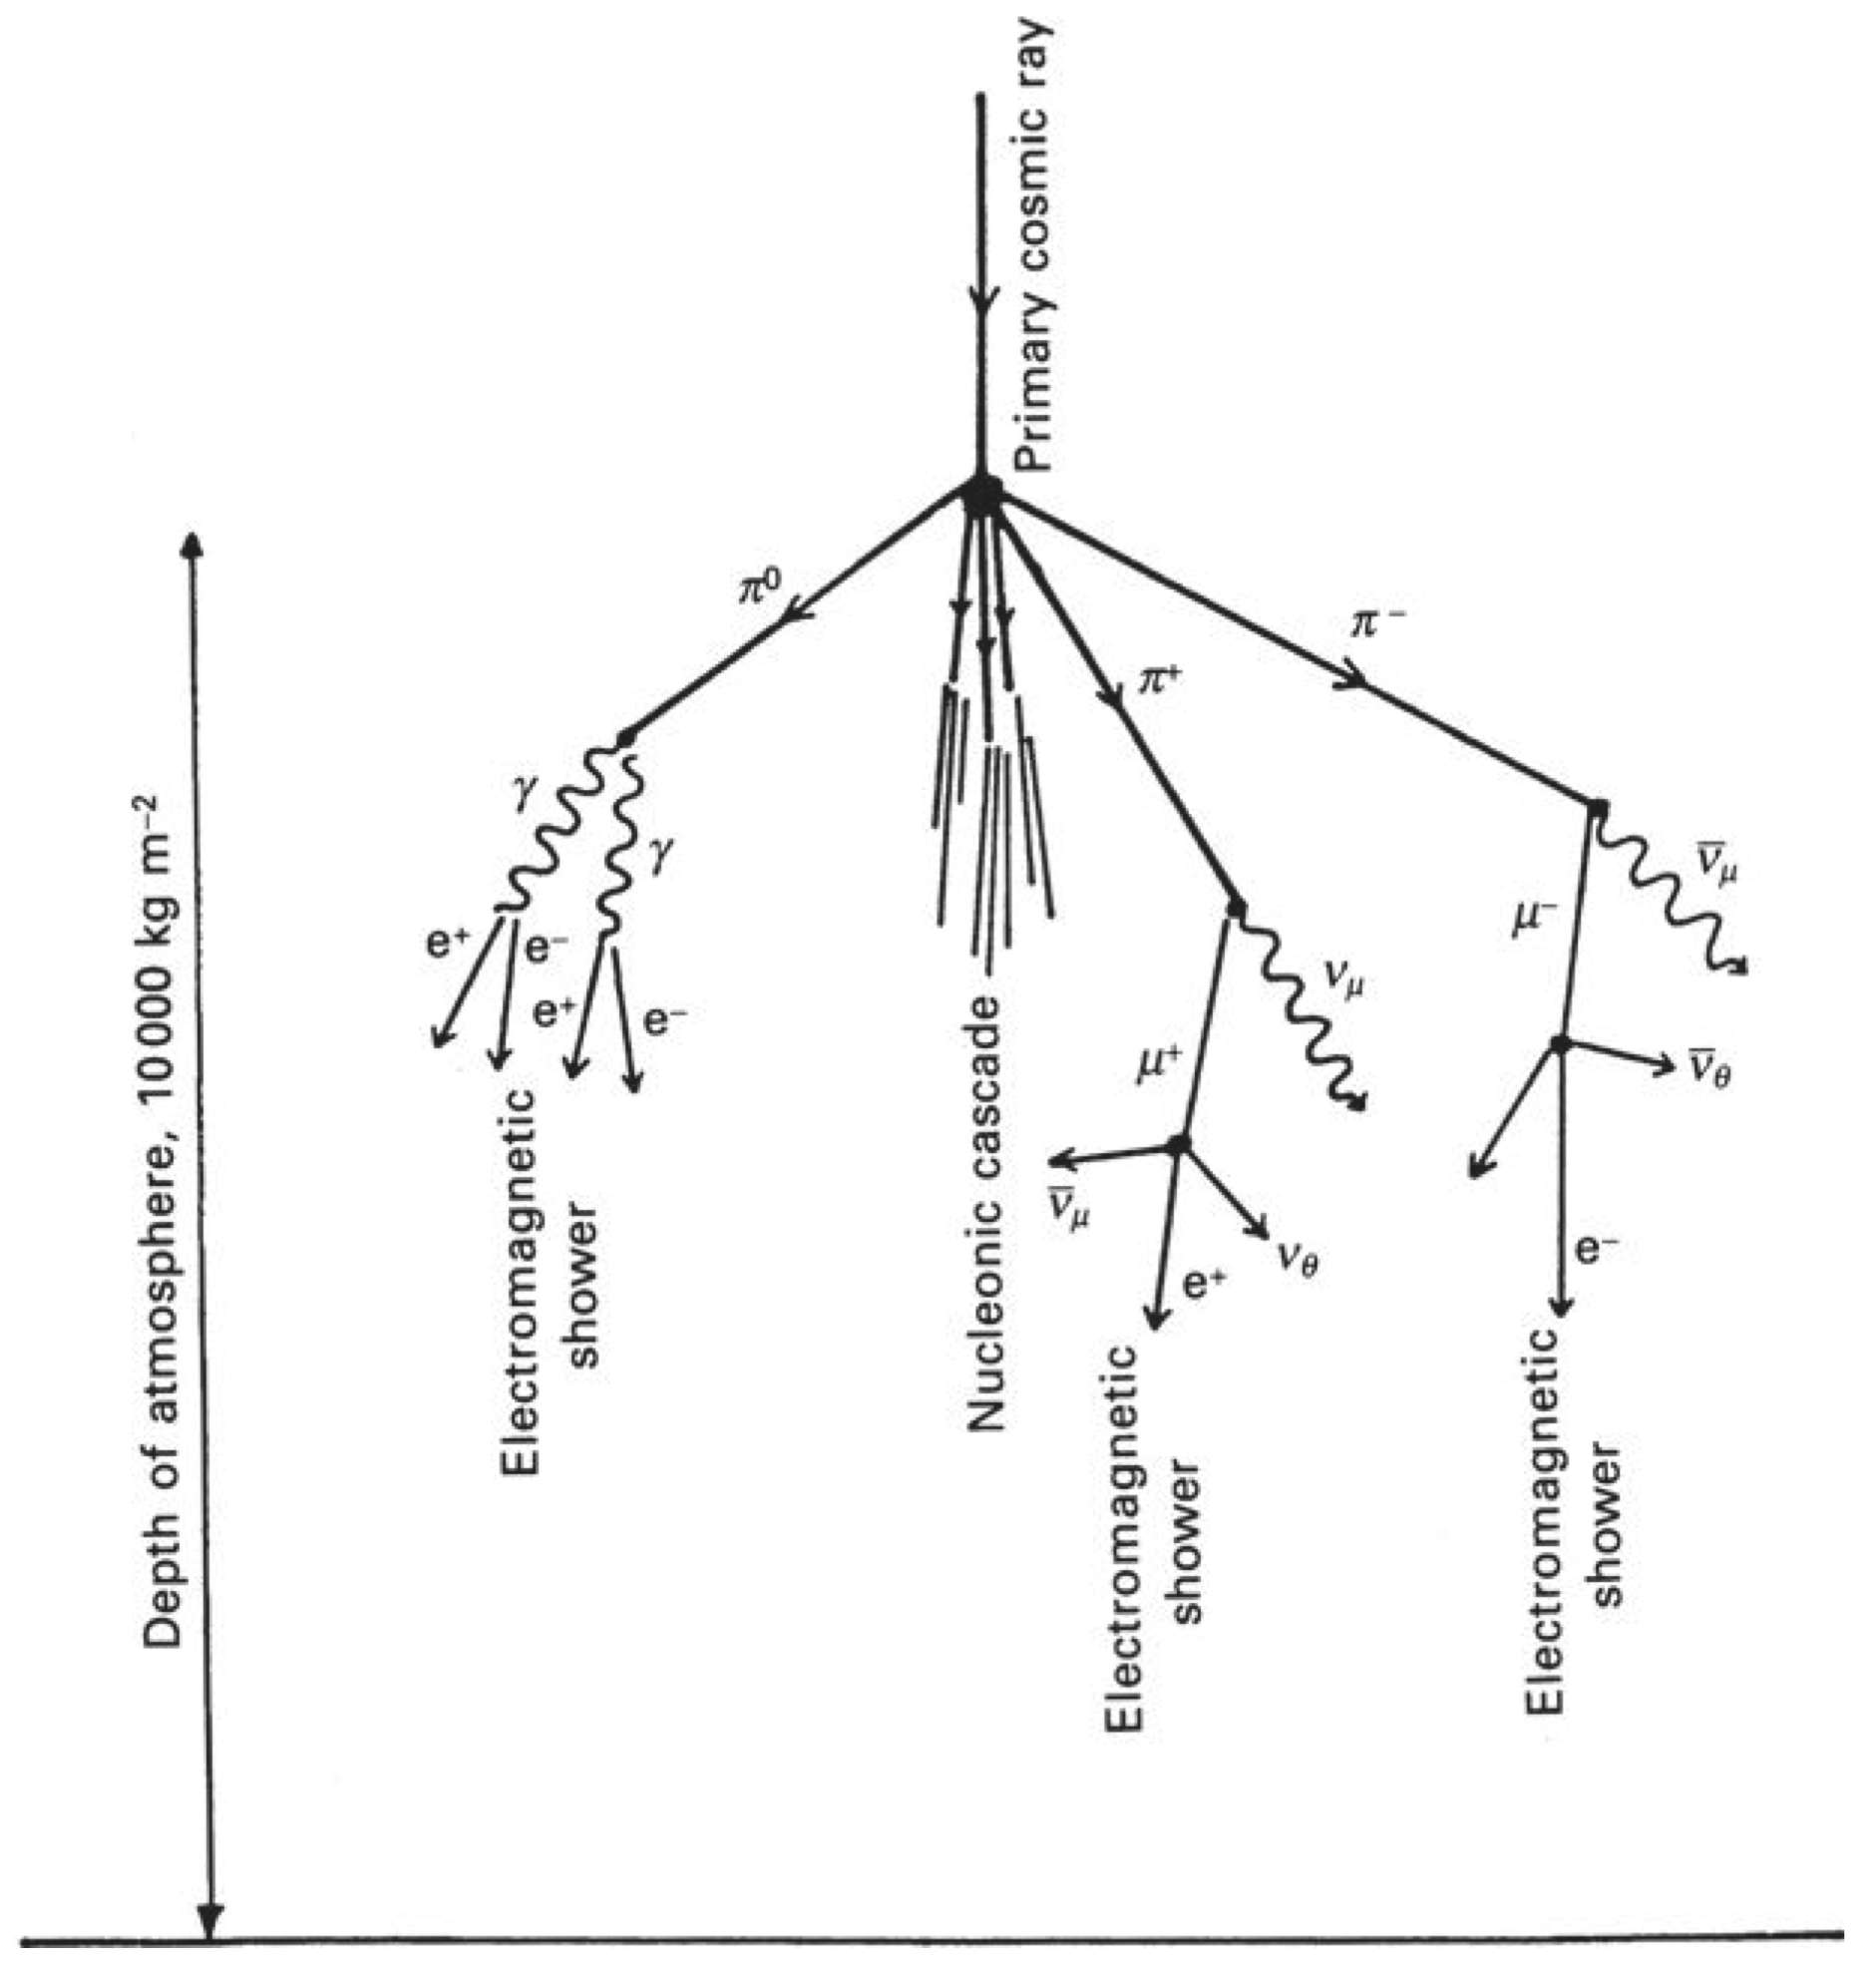
\includegraphics[width=0.7\linewidth]{figures/Muons/MuonShower.png}
    \caption{Diagram showing the interaction of a primary cosmic ray with nuclei in the upper Earth's atmosphere and the development of a nucleon cascade producing secondary cosmic rays in the form of muons, neutrinos and electromagnetic showers. Figure reprinted from Ref.\cite{Longair_2011}.}
    \label{fig:Muons/CRDiagram}
\end{figure}
As shown in \autoref{eqn:CREnergy}, the primary CR spectrum follows a power-law which is consequently applicable to the secondary CR products. However, the muon spectrum has added complexity as charged mesons interact with the atmosphere and in turn lose energy before decaying. T.K. Gassier proposed a parametrisation \cite{Gaisser_Engel_Resconi_2016} which results in an approximate formula for the muon spectrum at sea level:
\begin{equation}
    \label{eqn:MuonIntensitySurfaceEarth1}
    \frac{dI_\mu}{dE_{\mu0}d\Omega}\approx\frac{0.14\times E^{-\gamma}_{\mu0}}{\text{cm}^2\cdot\text{s}\cdot\text{sr}\cdot\text{GeV}}\times\Biggl\{\frac{1}{1+\frac{1.1\:E_{\mu0}\text{cos}\theta}{115\text{ GeV}}}+\frac{0.054}{1+\frac{1.1\:E_{\mu0}\text{cos}\theta}{850\text{ GeV}}}\Biggl\},
\end{equation}
where $\frac{dI_\mu}{dE_{\mu0}d\Omega}$ is the differential muon intensity at sea level, $E_{\mu0}$ is the muon energy at the Earth's surface and $\theta$ is the zenith angle of the muon at the surface (valid for $\theta<70^\circ$ accounting for the curvature of Earth). A spectral index, $\gamma=2.7$ was proposed by Gaisser \cite{Gaisser_Engel_Resconi_2016}. The two terms within the parentheses represent the muon produced from pion decay and kaon decay respectively, where the values of 115~GeV and 850~GeV correspond to the critical energies of these two particles. The critical energy is defined as the energy at which the probability of interaction is equal to the probability of decay at the height of a decay. The angular dependence of this term is because high energy pions will traverse less atmosphere before decaying into a high energy muon.
Taking into account the curvature of Earth and additional muon processes, \autoref{eqn:MuonIntensitySurfaceEarth1} is modified:
\begin{equation}
\label{eqn:MuonIntensitySurfaceEarth2}
\begin{split}    
    \frac{dI_\mu}{dE_{\mu0}d\Omega}(E_{\mu0},\theta^*)\approx&\frac{A\times 0.14\times (E_{\mu0}+\Delta E_{\mu0})^{-\gamma}}{\text{cm}^2\cdot\text{s}\cdot\text{sr}\cdot\text{GeV}}\\
    &\times\Biggl\{\frac{1}{1+\frac{1.1\:(E_{\mu0}+\Delta E_{\mu0})\text{cos}\theta_1}{115\text{ GeV}}}+\frac{0.054}{1+\frac{1.1\:(E_{\mu0}+\Delta E_{\mu0})\text{cos}\theta_1}{850\text{ GeV}}}+R_c\Biggl\}\times p_d,
\end{split}
\end{equation}
where $\frac{dI_\mu}{dE_{\mu0}d\Omega}(E_{\mu0},\theta^*)$ is the differential muon intensity at sea level, $E_{\mu0}$ is the muon energy at the surface, $\theta^*$ is the zenith angle at the surface, $\theta_1$ is the zenith angle at production of site of the muon in the atmosphere which relates to $\theta^*$ as follows, $\text{cos}\:\theta_1=\sqrt{1-0.99\cdot(1-\text{cos}^2\:\theta^*)}$, $\Delta E_{\mu0}$ is the muon energy loss in the atmosphere, $R_c=1\times10^{-4}$ is the ratio of muons to pions \cite{LVD:1998lir}, and $p_d$ is the probability for the muon not to decay in the atmosphere. The survival probability for high energy muons which reach deep underground labs is practically 1, so the precise parametrisation of the muon decay probability is not critical for underground muon physics.

The normalisation factor $A$ and the spectra index $\gamma$ can be chosen to fit experimental data and is dependent on depth. For depths $>2.5~\text{km}$ water equivalent (w.e.), the relation for `depth - vertical muon intensity' measured by the LVD experiment found $\gamma=2.77$ with a normalisation of the absolute flux $A=1.84$ found a good fit to data \cite{LVD:1998lir}.

\section{Muon transport through materials}\label{sec:Muons/MuonTransport}
As muons are charge particles they lose energy as they traverse materials through electromagnetic interactions with nuclei and atomic electrons in the medium. Energy loss through ionisation is the process where the passing charged particle (a muon in this particular case) transfers energy to the atomic electrons. The atom will either be excited or ionised depending on the proximity of the charged particle. The mean rate of energy loss of a muon due to ionisation and excitation can be described using the Bethe-Bloch formula:
\begin{equation}\label{eqn:BetheBloch}
    \Biggl<-\frac{dE}{dx}\Biggl>=4\pi\alpha^2N_A\frac{Z}{A}\frac{z^2(\hbar c)^2}{m_e^2v^2}\Biggl[\text{ln}\frac{2m_ev^2\gamma^2}{I}-\frac{v^2}{c^2}-\delta(\beta\gamma)\Biggl],
\end{equation}
where $\alpha=e^2/4\pi\epsilon_0\hbar c\approx1/137$ is the fine structure constant, $z$ is the charge of the muon (in units of electric charge), $\gamma=1/\sqrt{1-\frac{v^2}{c^2}}$ is the Lorentz factor, $v$ is the velocity of the muon with mass $m_\mu$ and energy $E$, $I\simeq16\:\cdot\:Z^{0.9}$ eV is the mean ionisation potential of the atom \cite{GROOM2001183}. As the energy of the muon increases, the electric field extends to large distances, increasing the number of interactions with distant electrons. This effect is corrected for in \autoref{eqn:BetheBloch} by the density correction term $\delta(\beta\gamma)$.

Muon additionally lose energy through radiative processes as discrete points of large energy loss. The total mean energy loss of the muon can be described as:
\begin{equation}\label{eqn:totMeanEnergyLossMu}
    \Biggl<-\frac{dE}{dx}\Biggl>=a(E)+b(E)E,
\end{equation}
where $x$ is the path length, $a(E)$ is the energy loss through ionisation as described with \autoref{eqn:BetheBloch}, and $b(E)$ is due to radiative
processes — bremsstrahlung, pair production, and photonuclear interactions:
\begin{equation}\label{eqn:radproc}
    b\equiv b_{\text{brems}}+b_{\text{pair}}+b_{\text{nucl}},
\end{equation}
where these three stochastic energy-loss processes with respect to charged particle are described briefly below:
\begin{itemize}
    \item \textbf{Bremsstrahlung:} As a charge particle passes near to the nucleus it decelerates, radiating a photon.
    \item \textbf{Pair-production:} Charged particles interact via the electromagnetic force, this interaction is mediated by a virtual photon, which in the field of the nucleus converts into a electron-positron pair.
    \item \textbf{Photonuclear interaction:} A photon radiated by the charged particle is absorbed by the nucleus and enters an excited state. The nucleus immediately decay releasing a hadron.
\end{itemize}
Both $a(E)$ and $b(E)$ are slowly varying functions of $E$, where at high energies losses by radiative processes dominate. The contributions from ionisation and radiative processes to the total stopping power of muons on copper is shown in \autoref{fig:Muons/StoppingPowerOffMuonsCu}. The critical energy, $E_{\mu c}$, is the energy at which the losses from ionisation and radiative processes are equal and is dependent on the material which the muon is propagating through.
\begin{figure}
    \centering
    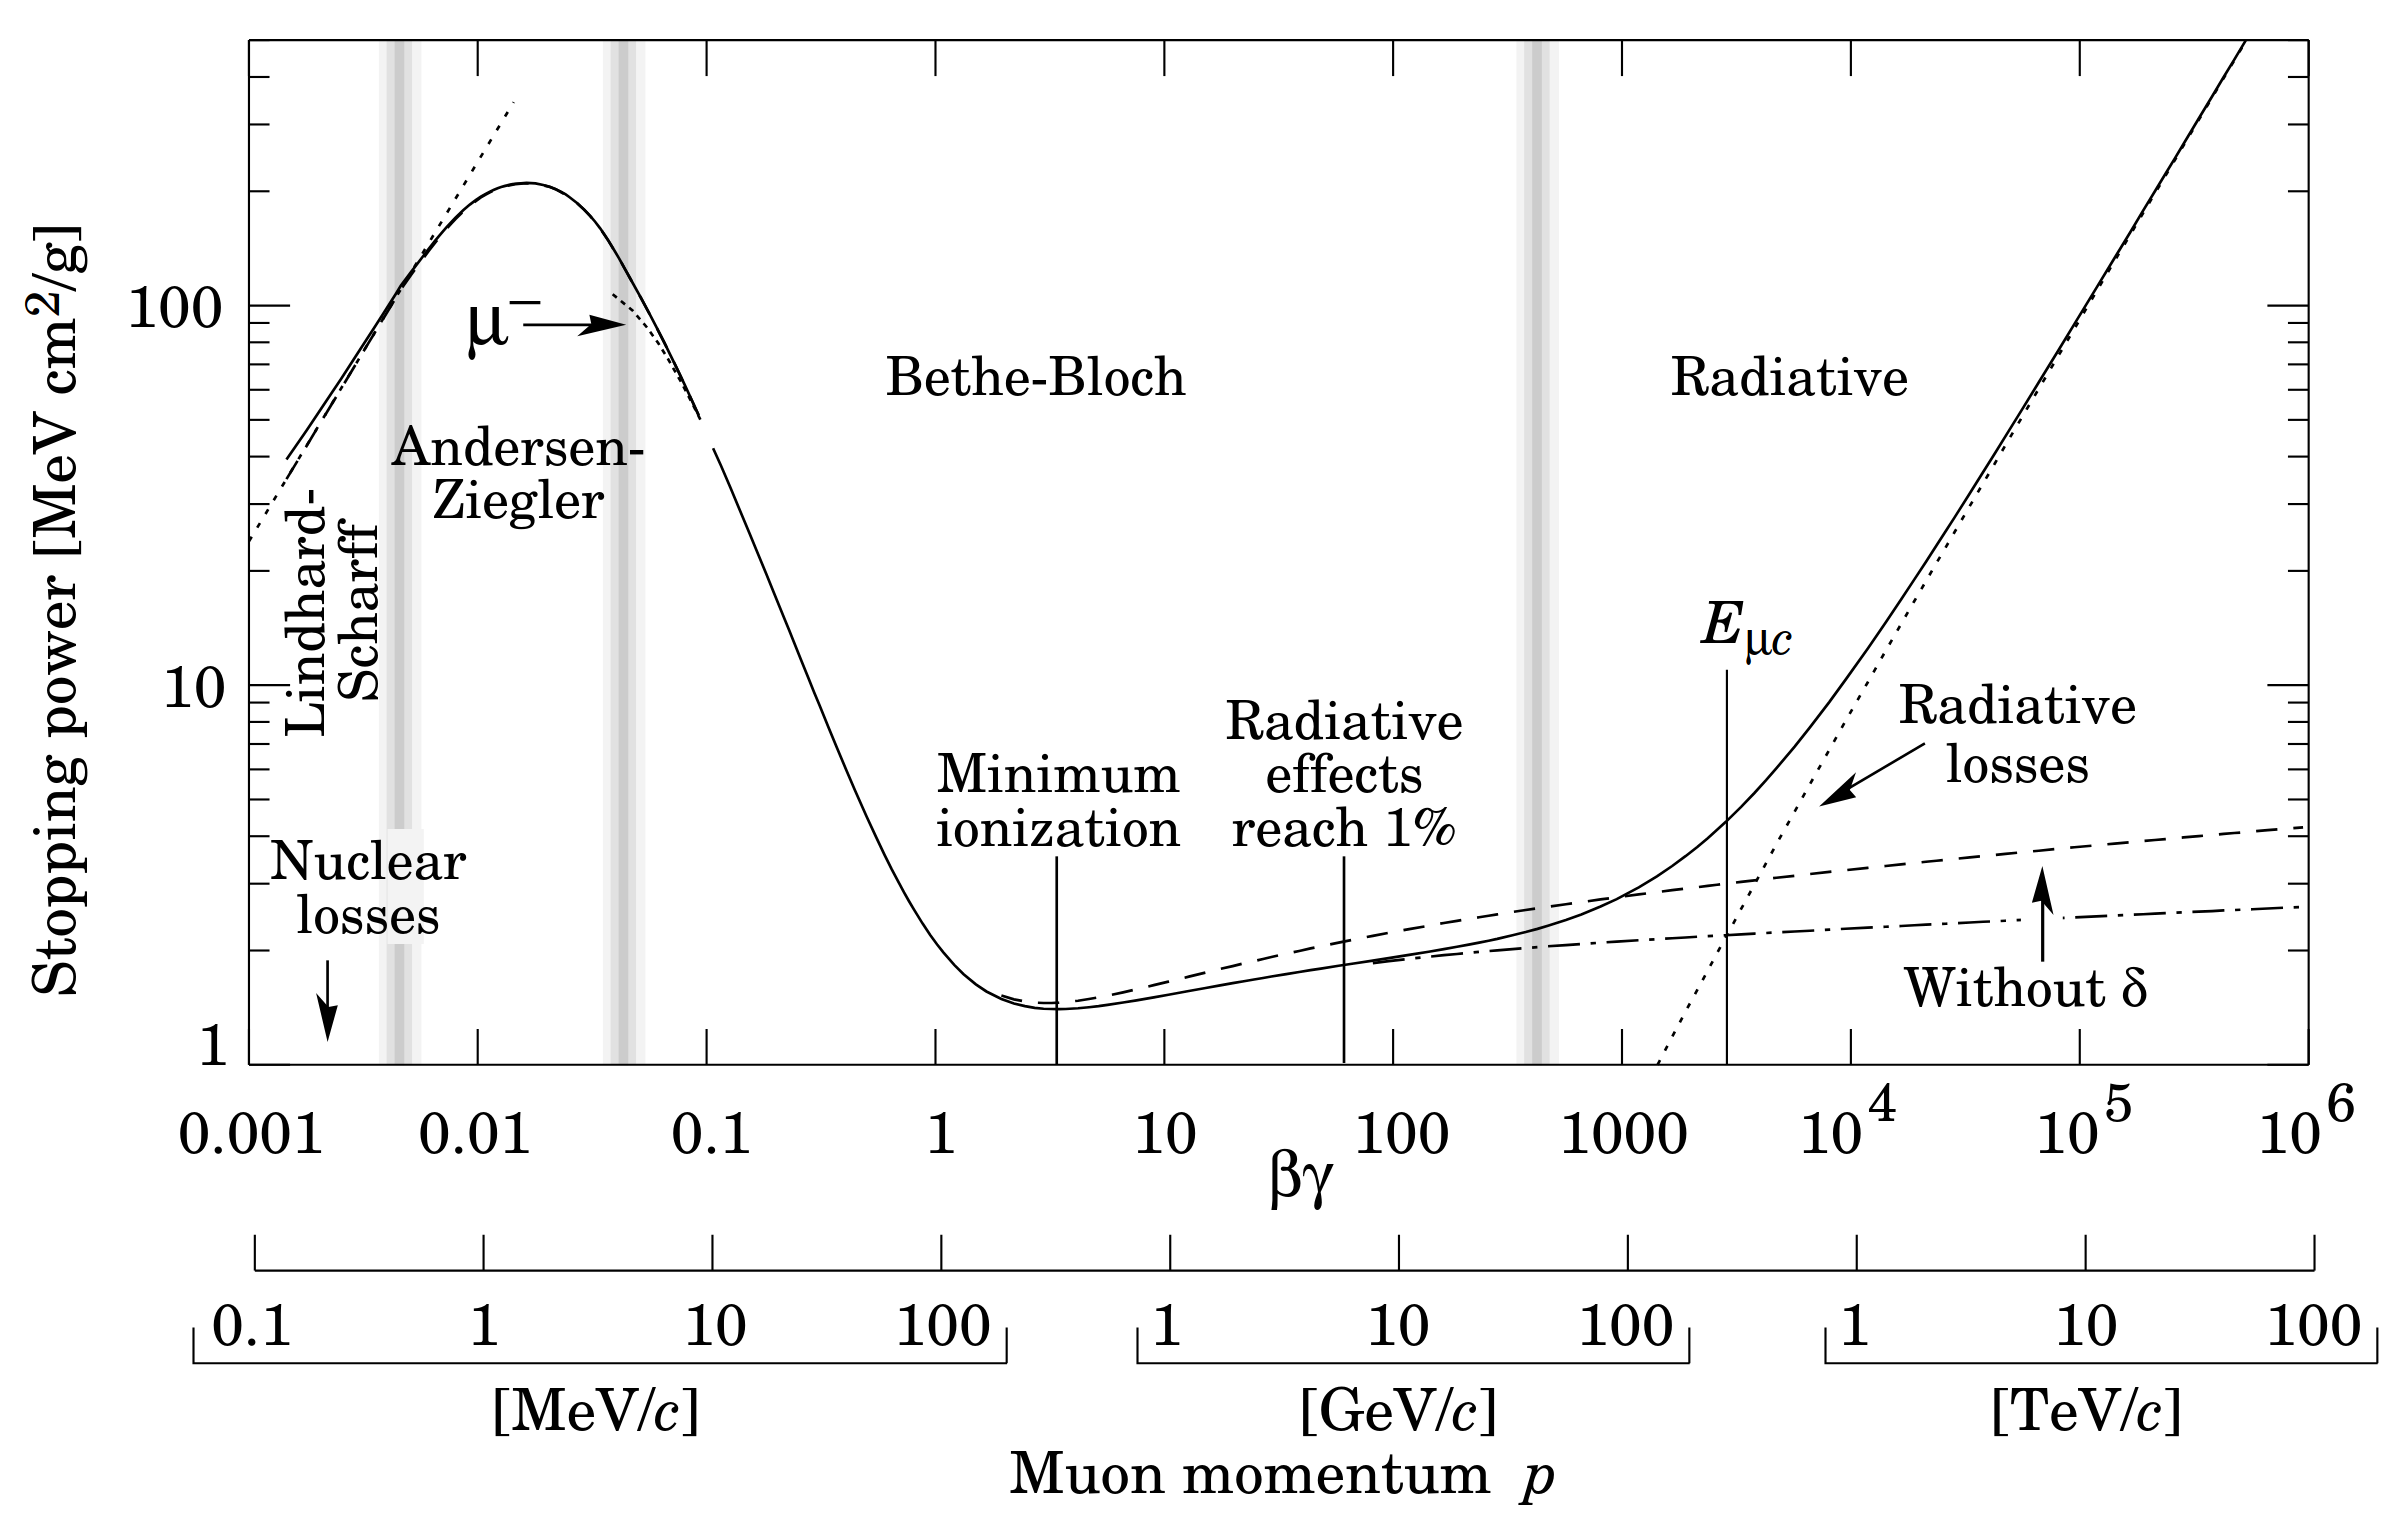
\includegraphics[width=0.9\linewidth]{figures/Muons/MassMuonStoppingPowerOfMuonsOnCu.png}
    \caption{Mass stopping power $\big<-dE/dx\big>$ for positive muons on copper as a function of $p=M\beta c\gamma$. Figure reprinted from Ref. \cite{GROOM2001183}.}
    \label{fig:Muons/StoppingPowerOffMuonsCu}
\end{figure}
In addition to the discussed energy loss processes, muons will also elastically scatter from nuclei via Coulomb interactions. However, the energy loss from this type of scattering can be consider negligible. As the muon propagates through a material, it will deviate from its track due to small angle deviations from the collective Coulomb scatters. 

\section{Muons underground}\label{sec:Muons/MuonsUnderground}
As a muon travels to from the surface to an underground site, the muon will undergo energy losses, as discussed in \autoref{sec:Muons/MuonTransport}. Depending on the energy of the incoming muon, it will either decay, be absorbed by the rock overburden, or reach the underground site. Due to this effect, muon intensity underground decreases with depth.

The muon spectrum underground can be described by \autoref{eqn:MuonIntensityUnderground}, which the convolution of the spectrum on the surface, (\autoref{eqn:MuonIntensitySurfaceEarth2}, and the probability for a muon with energy $E_{\mu 0}$ at the surface to have the energy $E_\mu$ at a depth $X$ \cite{musun}.
\begin{equation}\label{eqn:MuonIntensityUnderground}
    \frac{dI_\mu}{dE_\mu d\Omega}(dE_\mu d\theta)=\int^\infty_0P(E_\mu,X(\theta),E_{\mu0})\frac{dI_{\mu0}}{dE_{\mu0}d\Omega}(E_{\mu0},\theta^*)dE_{\mu 0}
\end{equation}
Simulation packages have been developed to model the passage of muons through large thicknesses of material to determine $P(E_\mu,X(\theta),E_{\mu0})$, one example which has been adopted by LZ is MUSIC (\textbf{MU}on \textbf{SI}mulation \textbf{C}ode) which has been extensively tested against experimental data and other packages \cite{musun,LVD:1998lir,PhysRevD.60.112001,Tang:2006uu,MACRO:2003qix}. The use of MUSIC alongside MUSUN (\textbf{MU}on \textbf{S}imulations \textbf{UN}derground) for muon simulations for LZ will be discussed in \autoref{sec:Muons/MuonFluxMeasurementWithLZ}.
The dependence of vertical muon intensity on depth for both water and rock is shown in \autoref{fig:Muons/MuonIntensityVSDepth}. Additional data on the total muon flux at various underground sites for equivalent depth relative to a flat overburden is summarized in \autoref{tab:MuonFluxVsDepth} and \autoref{fig:Muons/MuonFluxVsDepth}.
\begin{figure}[ht!]
    \centering
    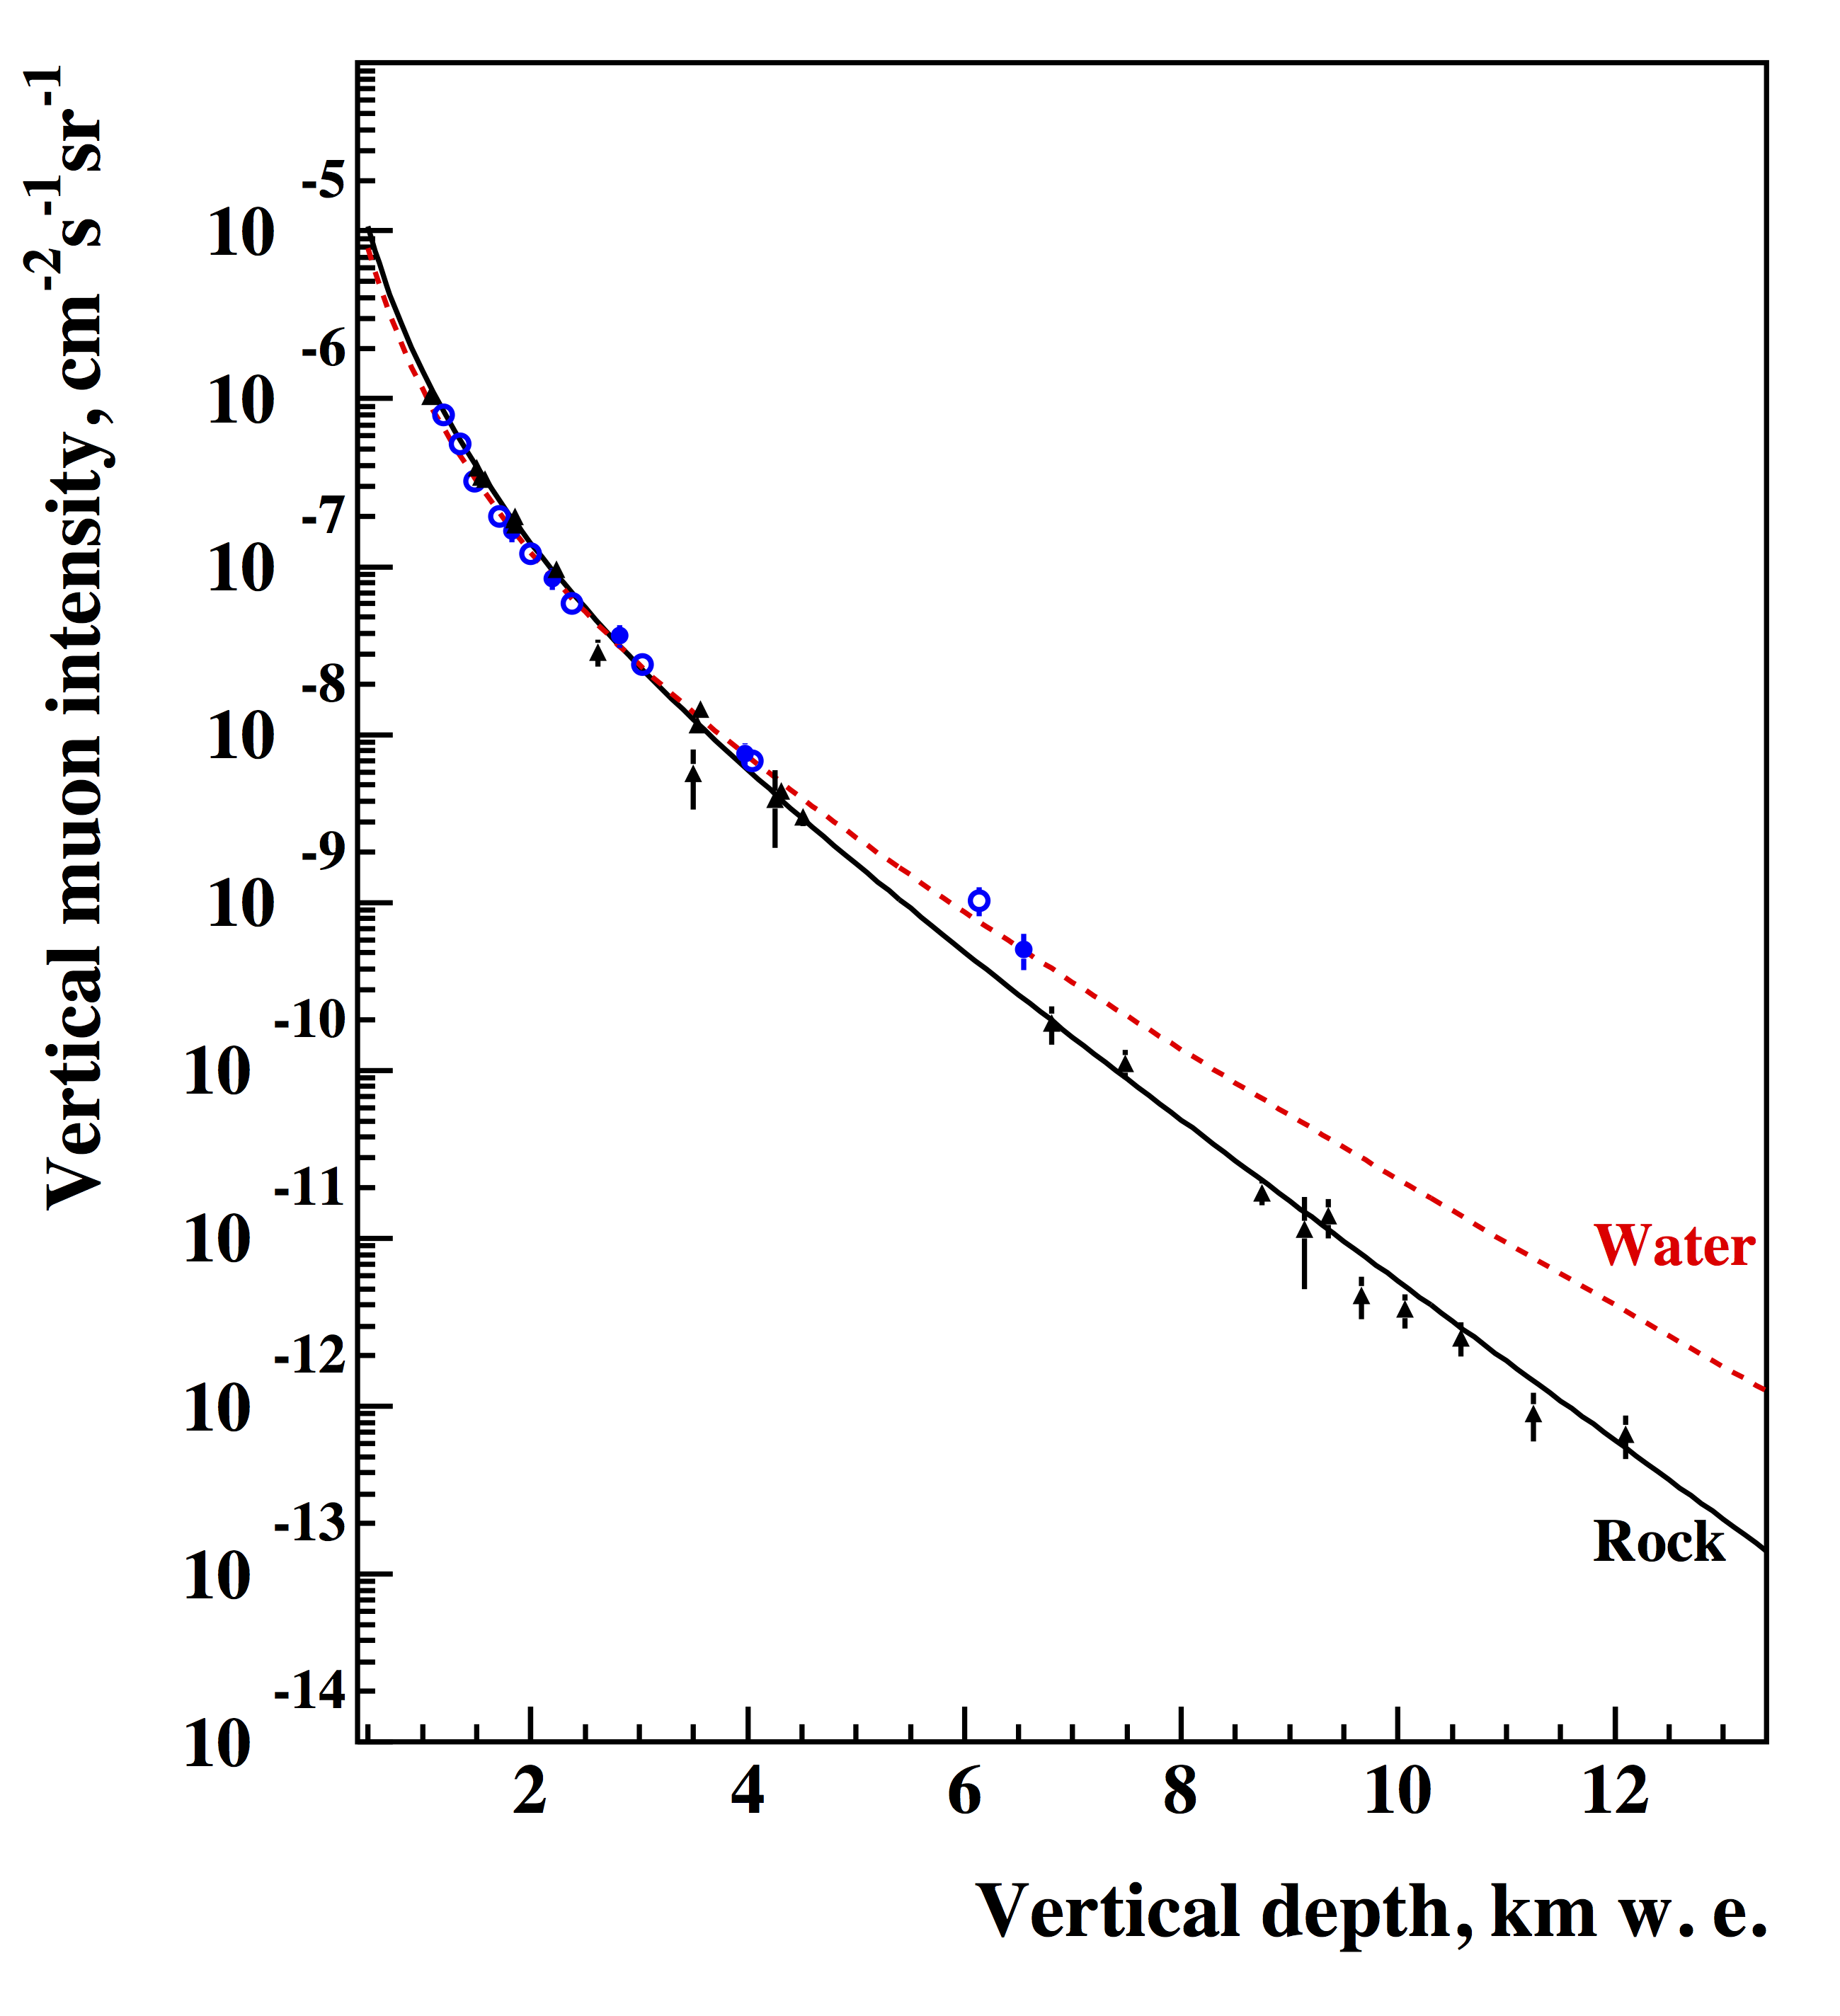
\includegraphics[width=0.7\linewidth]{figures/Muons/MuonIntensityVSVertDepth.png}
    \caption{Vertical muon intensity dependence on depth for standard rock ($<Z>\:=11$) and water. The filled triangles correspond to a collection of experiments with a rock overburden \cite{Kozyarivsky:1988gxn}. The open circles are data points taken the Baikal underwater neutrino telescope \cite{BAIKAL:1997iok}. Figured reprinted from Ref. \cite{dwoodward:thesis}.}
    \label{fig:Muons/MuonIntensityVSDepth}
\end{figure}
\begin{figure}[ht!]
    \centering
    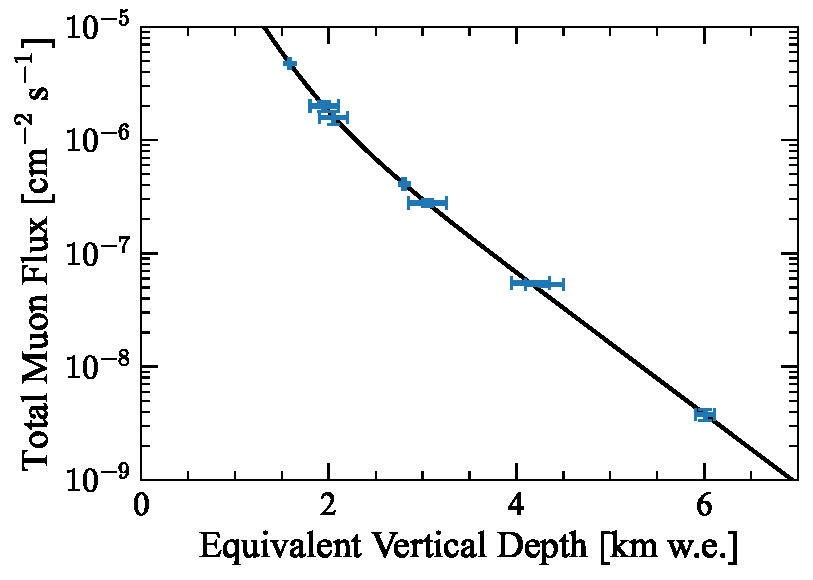
\includegraphics[width=0.7\linewidth]{figures/Muons/Flux_Depth_Plot.pdf}
    \caption{The total muon flux measured for different underground sites summarised in \autoref{tab:MuonFluxVsDepth} as a function of equivalent vertical depth relative to a flat overburden. The smooth curve is global fit function is described in Ref.\cite{mei}. Plot adapted from \cite{mei}.}
    \label{fig:Muons/MuonFluxVsDepth}
\end{figure}
\begin{table}[ht!]
    \centering
    \begin{tabular}{|c|c|c|}
        \hline
        Laboratory & Depth [km] & Muon flux [$\text{cm}^{-2}\text{s}^{-1}$]\\
        \hline
         WIPP & $(4.77\pm0.09)\times10^{-7}$ & $1.585\pm0.011$\\
         Soudan & $(2.0\pm0.2)\times10^{-7}$ & $1.95\pm0.15$\\
         Kamioka & $(1.58\pm0.21)\times10^{-7}$ & $2.05\pm0.15^\dagger$\\
         Boulby & $(4.09\pm0.15)\times10^{-8}$ & $2.805\pm0.015$\\
         Gran Sasso & $(2.78\pm0.2)\times10^{-8}$ & $3.05\pm0.2^\dagger$\\
         Fr\'ejus & $(5.47\pm0.1)\times10^{-9}$ & $4.15\pm0.2^\dagger$\\
         Homestake & $(5.31\pm0.17)\times10^{-9}$ & $4.3\pm0.2$\\
         Sudbury & $(3.77\pm0.41)\times10^{-10}$ & $6.011\pm0.1$\\
         \hline
    \end{tabular}
    \caption{Summary of the total muon flux measured at different underground sites and the equivalent vertical depth relative to a flat overburden ($^\dagger$ Equivalent vertical depth with flat overburden) Adapted from Ref.\cite{mei}.}
    \label{tab:MuonFluxVsDepth}
\end{table}

\section{Muon induced backgrounds}\label{sec:Muons/InducedBackgrounds}
Atmospheric muons which reach underground sites and traverse through a detector are detected as background events in the case of dark matter direct detection experiments. However, high-energy muons can be problematic to rare event searches since they produce secondary particles due to interactions with the rock overburden close to the detector and other material within and surrounding the detector. Muons which miss the detector but produce associated secondary particles may produce signal-like events. These such events cannot be rejected through coincidence with the incident muon \cite{mei,Lindote:2008nq}. Muon-induced neutrons, one such secondary particle, are particularly troublesome for dark matter detectors which cannot discriminate between single neutron interactions and dark matter candidates. The contribution of muon-induced neutrons to the total underground neutron flux in small \cite{LZ_SIMS}, however muon-induced neutrons have an energy spectrum up to several GeV. Fast neutrons with such energies are impervious to passive detector shield and interact with the detector. There are several processes which produce neutrons from high-energy muons:
\begin{equation}\label{eqn:MuonInt1}
    \mu^-+X\rightarrow X' + n+\nu_\mu
\end{equation}
\begin{equation}\label{eqn:MuonInt2}
    \mu^-+p\rightarrow n+\nu_\mu
\end{equation}
\begin{equation}\label{eqn:MuonInt3}
    \gamma+X\rightarrow X'+n
\end{equation}
\begin{equation}\label{eqn:MuonInt4}
    \pi+X\rightarrow X'+n
\end{equation} 
where $X$ and $X'$ represent the initial and final states of nuclei. \autoref{eqn:MuonInt1} represents neutron production via nuclear interactions caused directly by the muons through spallation. \autoref{eqn:MuonInt2} represents negative muon capture on a proton in the nucleus of the target atom. \autoref{eqn:MuonInt3} and \autoref{eqn:MuonInt4} represent products of muon-induced electromagnetic or hadronic cascades interacting with the nuclear of the target atom.

Negative muon capture is dependent on the ratio of stopping-muons to through-going muons. The rate of stopping-muons is energy dependent of incoming atmospheric muons due to the loss of momentum whilst travelling through rock and the production of secondary particles which the mechanisms discussed in \autoref{sec:Muons/MuonTransport}. Thus the rate of negative muon capture is only significant at depths $\lesssim100\text{m w.e.}$ \cite{Gaisser_Engel_Resconi_2016}. The rate of neutron production from electromagnetic and hadronic cascades is significantly larger than the rate of neutron production via muon-induced spallation at deep underground sites.

In general, the rate of muon-induced backgrounds is dependent on two factors, the depth of the underground site and the composition of the overburden material. To understand the effect that muon-induced background have on deep underground detectors and initial measurement of the muon flux through the detector in question must be made. The following sections discuss the muon flux measurement with the LZ experiment and their direct impact on data taking during the WS2022 and WS2024 WIMP search campaigns.  

\section{Muon flux measurement with the LUX-ZEPLIN experiment}\label{sec:Muons/MuonFluxMeasurementWithLZ}
Our initial muon model described in Ref.~\cite{LZ_SIMS} has been used to calculate muon fluxes that can be compared with previous measurements. Vertical muon intensity has been calculated as $5.18\times10^{-9}$~cm$^{-2}$~s$^{-1}$~sr$^{-1}$, in good agreement with the value of $(5.38\pm0.07\text{ (stat)})\times10^{-9}$~cm$^{-2}$~s$^{-1}$~sr$^{-1}$~\cite{Cherry} measured in the same cavern using the veto system of the Davis experiment. Total muon flux through a spherical detector with unit cross-sectional area has been calculated as $6.16\times10^{-9}$~cm$^{-2}$~s$^{-1}$, slightly higher than the recent measurements with the veto system of the Majorana Demonstrator located in the nearby cavern $(5.31\pm0.17 \text{ (stat)})\times10^{-9}$~cm$^{-2}$~s$^{-1}$~\cite{majorana}.\\
The difference between the two measurements and our initial model, although relatively small (within 20\%), pointed to a need for new measurements with the LZ experiment to re-normalise the muon model.\\
The new muon flux measurements estimate the average density of the rock between the surface and the cavern and will be used to inform the muon model for the DUNE experiment\cite{DUNE}, which uses the same MUSUN code and the same rock density.

\subsection{Outline of model}\label{sec:Muons/ModelOutline}
The muon simulations use two Monte-Carlo codes: MUSIC (\textbf{MU}on \textbf{SI}mulation \textbf{C}ode) and MUSUN (\textbf{MU}on \textbf{S}imulations \textbf{UN}derground)\cite{music,musun}, adapted here for the LZ experiment. Initially, muons with different energies on the surface of the Earth were transported through various distances in rock using MUSIC. The rock composition has been taken from Ref.~\cite{mei,zhang}. Measurements of several rock samples have been reported~\cite{mei,zhang} and the average rock parameters have been calculated as $<Z>=12.09$ and $<A>=24.17$. The average density of rock was assumed to be 2.70 g/cm$^3$~\cite{zhang} in the MUSIC simulation. Other measurements \cite{heise}, including the measurement of the muon flux with the veto system of the Majorana demonstrator, suggest that the density may be larger (2.8-2.9 g/cm$^3$\cite{majorana}).

The resulting energy spectra of survived muons have been convoluted with muon spectra on the surface of the Earth for different zenith angles and slant depths (see~\cite{musun} for the procedure's description). The distance from the underground laboratory and the Earth's surface for each azimuth and zenith angle has been obtained from the surface map and the position of the laboratory in the global coordinate system~\cite{richardson}.
Muon energy spectrum and zenith angle distribution on the surface of the Earth were calculated using the parametrisation first suggested in Ref.~\cite{Gaisser_Engel_Resconi_2016} modified for the curvature of the Earth to include large zenith angles. Other corrections, such as muon decay and energy loss in the atmosphere, muon production via charmed meson decay, muon intensity dependence on altitude and geomagnetic rigidity cut-off were not included due to their negligible effect on high-energy muons ($>1$~TeV) capable of reaching the SURF location.
As a result of muon transport and convolution with the surface fluxes, muon energy spectra and different angles at the detector site have been calculated and stored in a file. The model gives the total muon flux through a sphere as $6.16\times10^{-9}$~cm$^{-2}$~s$^{-1}$, mean muon energy of 283~GeV, mean zenith angle of 27$^{\circ}$ and the mean slant depth of 4500~m~w.~e.~\cite{musun-lz}.

The Muon generator MUSUN inside BACCARAT reads muon distributions from this file and samples muons on the horizontal (top) and vertical surfaces of a box that encompasses the laboratory hall. The top horizontal surface of the box is located 7 metres above the cavern boundary. Vertical surfaces of the box are positioned 5 m away from the boundary. The box extends to 3 m below the cavern floor. Moving the box surfaces into the rock, away from the cavern, ensures the development of muon-induced cascades in rock or shotcrete before muons and their secondaries enter the cavern. The primary energy spectrum and the angular distributions of these muons are illustrated in \autoref{Prime_info}.

\begin{figure*}[htbp]
    \centering
    \begin{subfigure}[b]{0.48\textwidth}
        \centering
        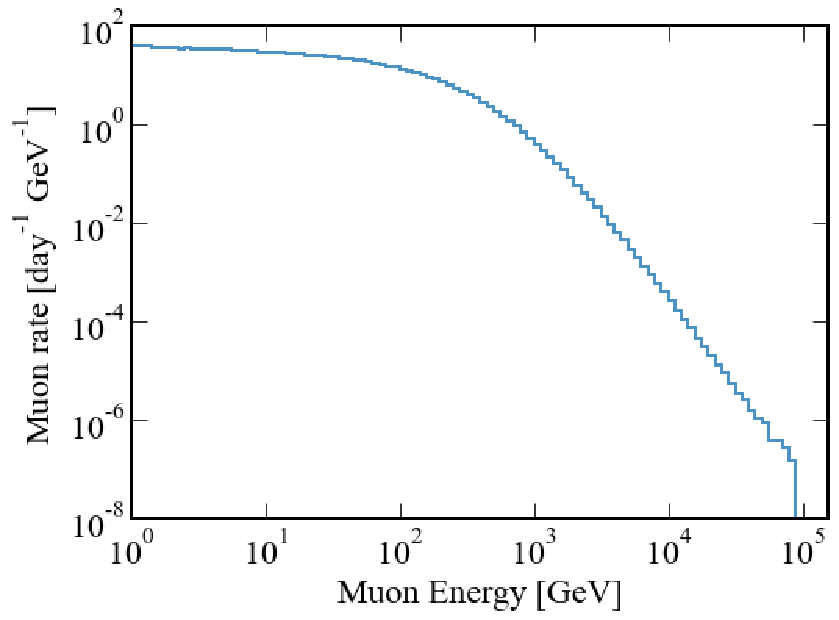
\includegraphics[width=\textwidth]{figures/Muons/Primary_energyLZstyle.pdf}
        \caption{Muon energy spectrum sampled from MUSUN.}
        \label{fig:Muons/Prim_E}
    \end{subfigure}
    %\hfill
    \begin{subfigure}[b]{0.49\textwidth}  
        \centering 
        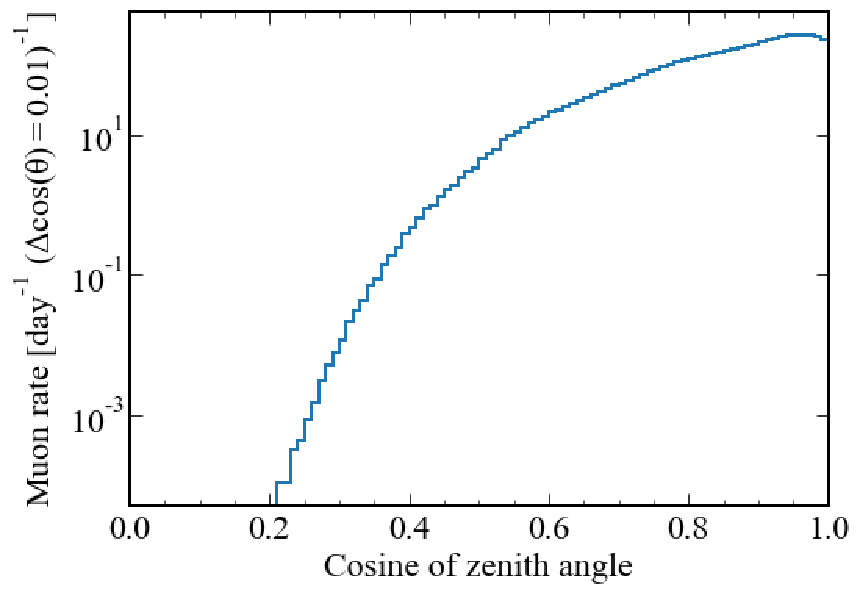
\includegraphics[width=\textwidth]{figures/Muons/cosZ_LZstyle.pdf}
        \caption{Zenith angle distribution of muons sampled from MUSUN.}
        \label{fig:Muons/cosZ}
    \end{subfigure}
    %\vskip\baselineskip
    \begin{subfigure}[b]{0.49\textwidth}   
        \centering 
        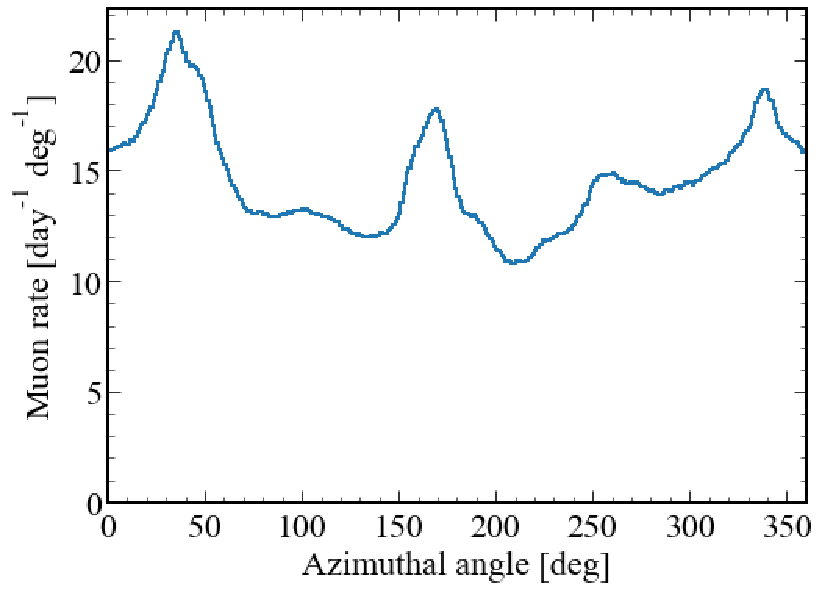
\includegraphics[width=\textwidth]{figures/Muons/Azimuthal.pdf}
        \caption{Azimuth angle distributions of muons counted East to North.}
        \label{fig:Muons/azi}
    \end{subfigure}
   % \hfill
    \begin{subfigure}[b]{0.49\textwidth}   
       % \vspace{-7mm}
        \centering 
        \includegraphics[width=\textwidth]{figures/Muons/SurfaceTopography.png}
        \caption{Surface altitude profile of the area above the Davis Cavern surrounding SURF. Figure reprinted from \cite{dwoodward:thesis}.} 
        \label{Azi_vs_Zen}
    \end{subfigure}
    \caption{Angular distributions and the kinetic energy spectrum of muons at SURF, Davis Campus, as generated by the MUSUN model.} 
    \label{Prime_info}
\end{figure*}
\par Muons generated by MUSUN have been transported through the rock, laboratory hall and detector geometry using GEANT4 (inside BACCARAT) and their energy depositions in all "sensitive volumes" have been recorded. In this simulation, $4.82\times10^7$ muons have been propagated which corresponds to a live time of 9147 days (0.0609874 muons per second), providing about 30 times higher statistics than for data collected during WIMP search 2022 and WIMP search 2024 (WS2022 \& WS2024).

\subsection{Data selection}\label{sec:Muons/MuonFluxDataSelection}
This study considers the both WS2022 and WS2024 datasets, specifically using the file lists, {\fontfamily{qcr}\selectfont SR1-WSv5\_LZAP-5.4.6.files.list}, taken from the {\fontfamily{qcr}\selectfont SR1WS} ALPACA module and {\fontfamily{qcr}\selectfont SR3-WSv8\_LZAP-5.8.0\_all.files.list }, taken from the {\fontfamily{qcr}\selectfont SR3LENR} ALPACA module. 

Skims of the data sets were performed using the {\fontfamily{qcr}\selectfont MuonPhys} ALPACA module which applied a loose initial selection to reduce the size of the initial dataset for later analysis. This module was also used for determining the live time of the two datasets. The live times are summarised in \autoref{tab:livetimes}. For the rate calculation, DAQ live time was chosen as the appropriate live time to use as this analysis is does not consider the same decision logic as used in the physics live time.

\begin{table}[htbp]
    \centering
    \caption{Summary if relevant durations for the WIMP search runs. For this analysis, DAQ livetime was used in the rate calculation work.}
    \begin{tabular}{|c|c|c|c|}
        \hline
        \textbf{Run} & \textbf{Run Time [days]} & \textbf{DAQ Live Time [days]} & \textbf{Physics Live Time [days]} \\
        \hline
        WS2022 & 99.5 & 98.8 & 96.4 \\
        WS2024 & 268.0 & 267.6 & 255.4 \\
        Total & 367.5 & 366.4 & 351.8 \\
        \hline
    \end{tabular}
    \label{tab:livetimes}
\end{table}

\subsubsection{Typical muon event}
\begin{figure}[htbp]
    \centering 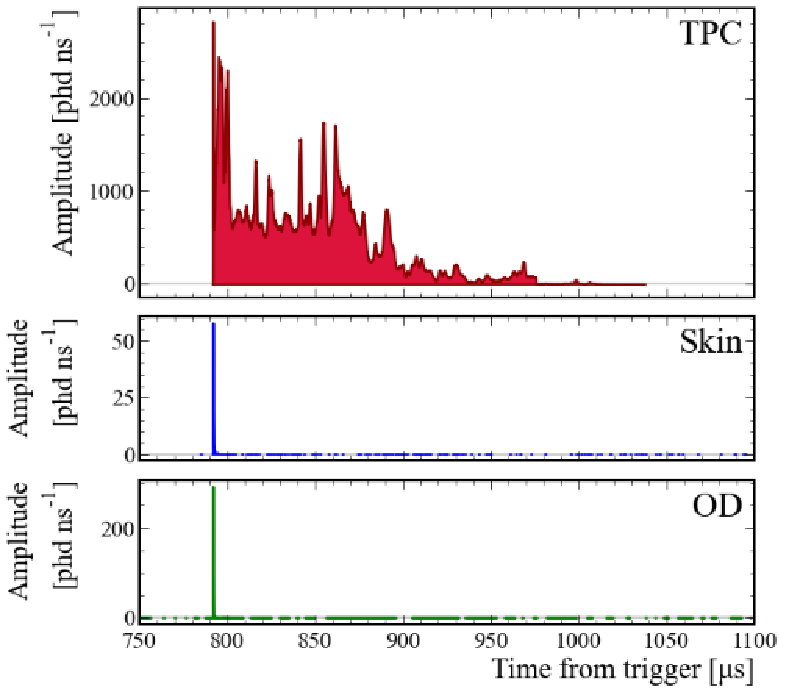
\includegraphics[width=0.7\textwidth]{figures/Muons/LZap_waveform.pdf}
    \caption{Event-viewer output of typical muon event. PMT saturation is evident towards the end of the muon ‘tail’ in the TPC.}
    \label{fig:Muons/eventViewer}
\end{figure}

\subsubsection{Outer detector selection}\label{sec:Muons/MuonFluxODSelection}
An OD energy threshold was implemented to reduce the probability of random coincidence between the three detectors. The energy deposited in the OD by a muon is the largest, physical signal we will see in the OD. The only other large physical signals we anticipate seeing are neutron captures, the most frequent of which are on gadolinium. Therefore, the OD threshold was set at the endpoint of the gadolinium neutron capture at $\sim$~8~MeV which corresponds to 2000~phd.
 % See \autoref{fig:Muons/ODPASpectra} which shows the Gd neutron capture spectra from 10 million events in background data during WS2022.
An OD `noise cut', initially developed for the muon veto and `hold off' for the WIMP search, has been used to reduce the impact of burst noise in our flux measurement. During tests of the muon veto, it was found that pulses produced due to the burst noise phenomena could imitate a muon-like signal in the OD. The ratio of pulse area to pulse amplitude enabled the creation of a custom variable called `Pulse Shape'.
Two distinct distributions can be seen in \autoref{fig:Muons/ODcut_pre}. Events from both distributions were hand scanned using the event-viewer and it was found that pulses with a pulse shape less than 0.003 were noise pulses with the same characteristics as previously observed burst noise. 
\begin{figure}[htbp]
    \centering
    \begin{subfigure}{0.49\textwidth}
    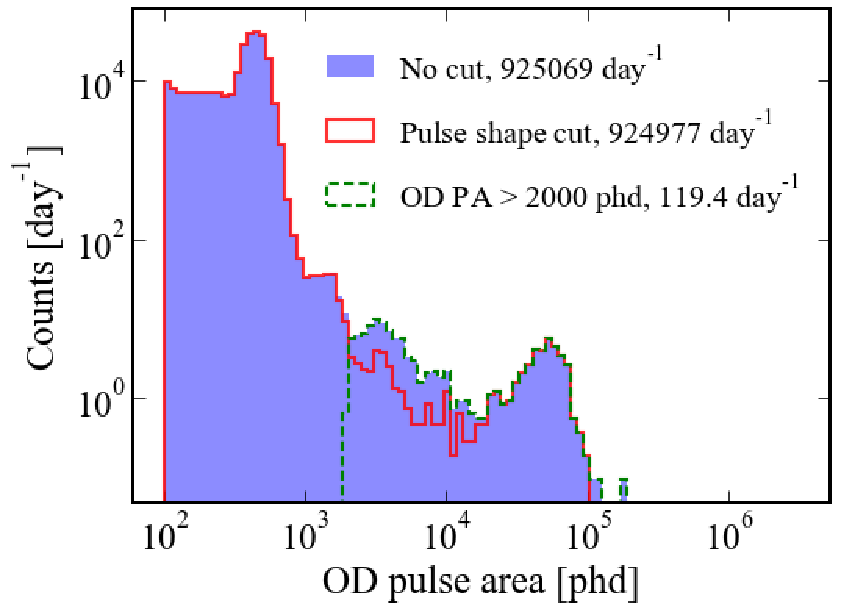
\includegraphics[width=\textwidth]{figures/Muons/OD_cuts_pre_coincidenceLZstyle.pdf}
    \caption{}
    \label{fig:Muons/ODcut_pre}
    \end{subfigure}
    \begin{subfigure}{0.49\textwidth}
    \centering
    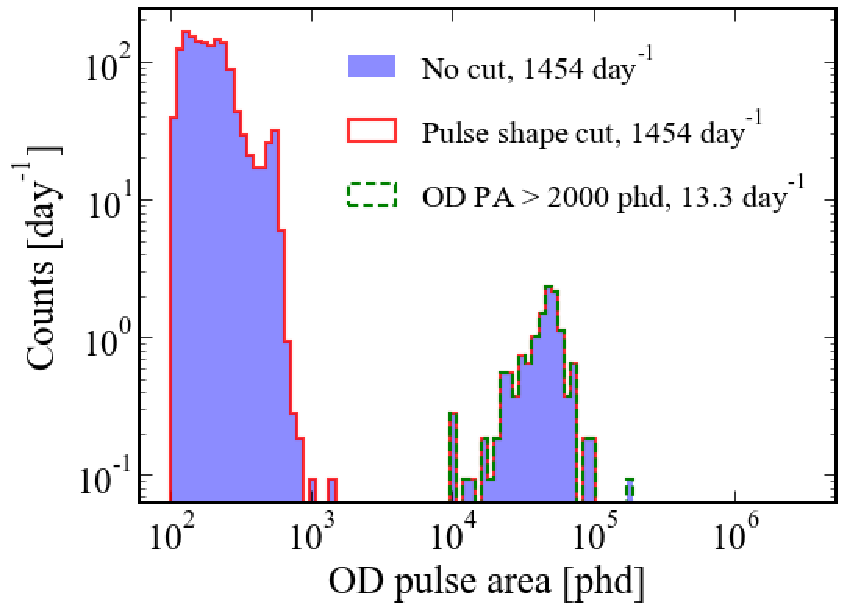
\includegraphics[width=\textwidth]{figures/Muons/OD_cuts_post_coincidenceLZstyle.pdf}
    \caption{}
    \label{fig:Muons/ODcut_post}
    \end{subfigure}
    \caption{%A histogram displaying the OD pulse area of the largest pulse areas in each of $\sim$12.5 million events from background data taken during WS2022, before inter-detector timing cuts are applied. 
    Histograms of the largest OD pulse areas in $\sim$12.5 million background events from WS2022 before applying inter-detector timing cuts. Pulse shape has been used to differentiate between pulses produced by a muon and pulses produced by noise phenomena observed in the detector. The peak at around 450~phd results from neutron captures on the nuclei of hydrogen atoms and the subsequent emission of a single 2.22~MeV gamma ray. The plots show the impact of the 2000~phd cut and pulse shape cut (a) before and (b) after inter-detector timing coincidences are applied.}%The characteristic hydrogen capture peak can be seen at \(\sim \)420~phd and then 
    \label{fig:Muons/ODSpectra}
\end{figure}

\subsubsection{Inter-detector timing selection}\label{sec:Muons/MuonFluxTimingSelection}
Atmospheric muon events in the LZ experiment can be uniquely identified by their large energy deposits that are coincident in the three detector systems: OD, skin and TPC. As muons move at relativistic speeds, the time difference between pulses in each detector will be small compared to other backgrounds such as neutrons and gamma rays.
Broad scans were conducted to make use of the coinciding detector signals to determine the inter-detector timing selection. As shown in \autoref{fig:Muons/timing_plots}, the time difference distributions between detector volumes allow for distinguishing between muon interactions through all volumes and signals unrelated to muons. Following the scan, three different considerations were made:
 \begin{enumerate}
    \item $-200~\text{ns} < \Delta t_{\text{OD - Skin}} < 200~$ns
    \item $-1200~\text{ns} < \Delta t_{\text{OD - TPC}} < 200~$ns
    \item $-1200~\text{ns} < \Delta t_{\text{Skin - TPC}} < 200~$ns
\end{enumerate}
Here the pulse time, $t$, is described using the combination of two RQs, \texttt{pulseStartTime\_ns} and \texttt{areaFractionTime5\_ns}. When traversing the TPC, a muon does not produce a singular pulse as observed in the OD and Skin. The muon ionises xenon atoms along the track, and a subsequent series of S1 and S2 pulses are produced. The pulses combine to produce a `tail' as seen in \autoref{fig:Muons/eventViewer}. The first pulse in the tail is used in the inter-detector timing selection. \autoref{fig:Muons/ODcut_post} highlights the effectiveness of the timing cut when used with the Outer Detector selection, reducing the event rate per day from 119.4 to 13.3.

\begin{figure}[htbp]
\centering
\begin{subfigure}{0.5\textwidth}
    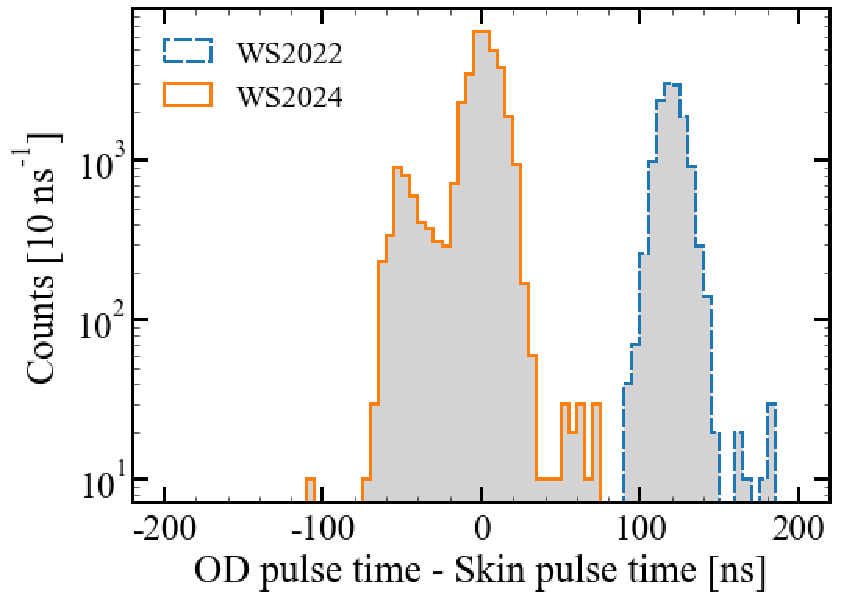
\includegraphics[width=\textwidth]{figures/Muons/OD-Skin_timing.pdf}
    \caption{}
    \label{fig:Muons/OD-Skin}
\end{subfigure}
\hfill
\begin{subfigure}{0.5\textwidth}
    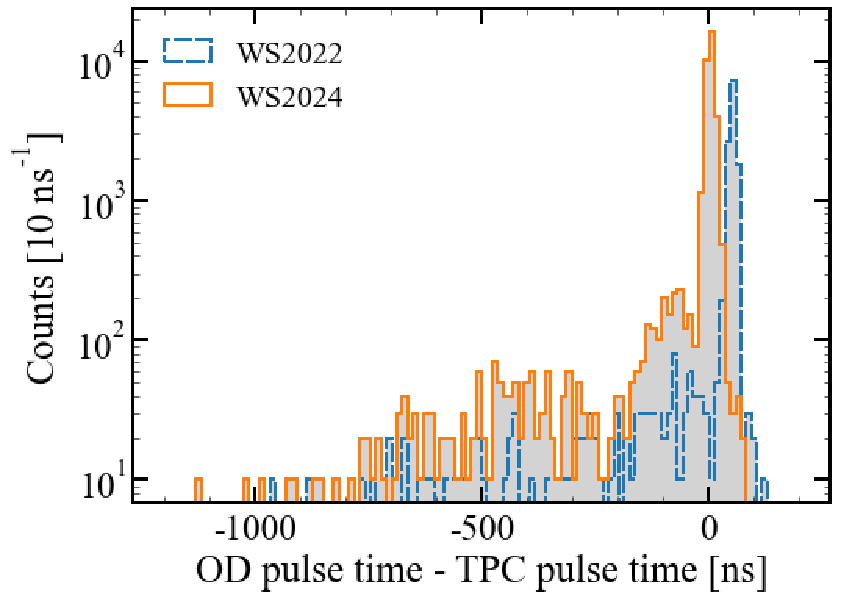
\includegraphics[width=\textwidth]{figures/Muons/OD-TPC_timing.pdf}
    \caption{}
    \label{fig:Muons/OD-TPC}
\end{subfigure}
\hfill
\begin{subfigure}{0.5\textwidth}
    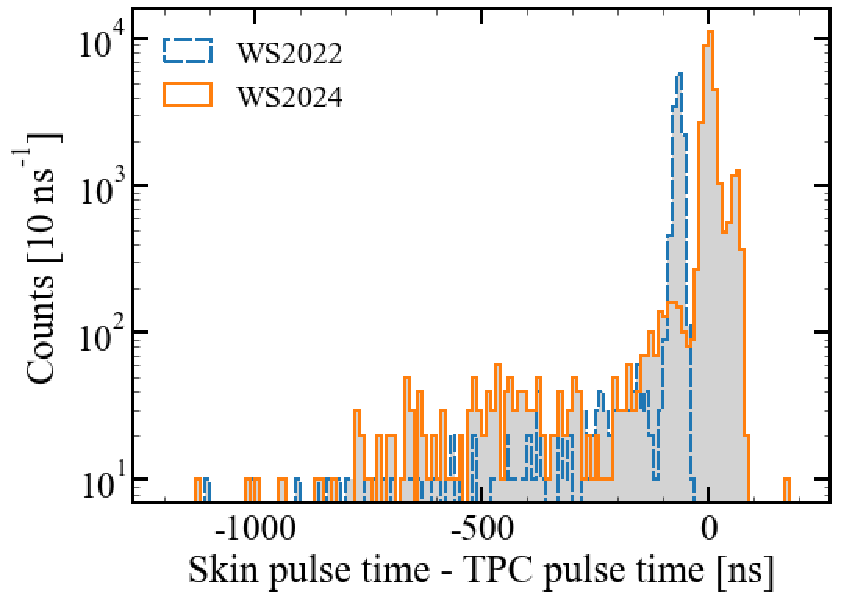
\includegraphics[width=\textwidth]{figures/Muons/Skin-TPC_timing.pdf}
    \caption{}
    \label{fig:Muons/Skin-TPC}
\end{subfigure}
\caption{Inter-detector timing plots, these distributions were used in defining the timing selection following the skim of the WS2022 and WS2024 datasets looking at events with a pulse greater than 2000~phd in the Outer Detector. The figures depict (a) the time difference between the largest pulse in the Outer Detector and the largest pulse in the Skin; (b) the time difference between the largest pulse in the Outer Detector and the start of the muon tail in the TPC; and (c) the time difference between the largest pulse in the Skin and the start of the muon tail in the TPC.}
\label{fig:Muons/timing_plots}
\end{figure}

\subsubsection{TPC energy selection}\label{sec:Muons/TPCEnergySelection}
The effects of cuts differ between simulations and data due to uncertainty associated with GEANT4 modelling of the muon shower, particularly at lower energies (see \autoref{fig:Muons/TPCHGLGComp_energy}). As the cuts change, the rates change accordingly, but by different factors for data and simulations. This difference can be observed by examining the ratios of muon flux between the data and the simulations. Therefore, two decisions are required: which gain (high gain, HG, or low gain, LG) should be used for data to normalise the muon model, and what threshold is necessary for energy deposition in the TPC to ensure that the data can be accurately compared with the simulations. To accomplish this, we worked backward from the flux results described in \autoref{sec:Muons/MuonRateResults}. Comparing HG ratios of data rates to simulated rates with the corresponding LG ratios, as displayed in \autoref{fig:Muons/TPCHGLGComp_ratios}, it is clear that the LG ratios remain steady within statistical errors above 10~MeV. 
\begin{figure}[htbp]
    \begin{subfigure}{.49\textwidth}
    \centering
    \centering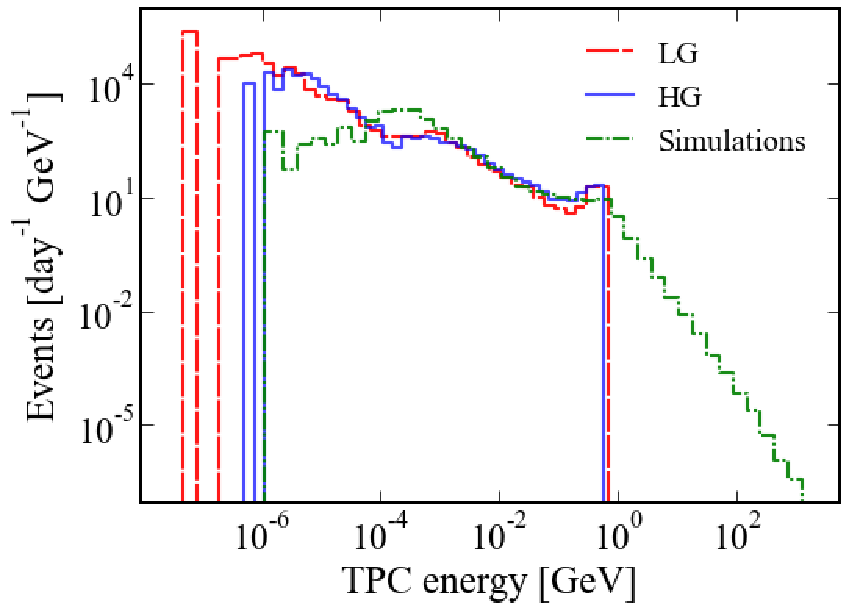
\includegraphics[width=1\textwidth,angle=0]{figures/Muons/TPC_energy_comp.pdf}
    \caption{}
    \label{fig:Muons/TPCHGLGComp_energy}
    \end{subfigure}
    \begin{subfigure}{.49\textwidth}
    \centering
    \centering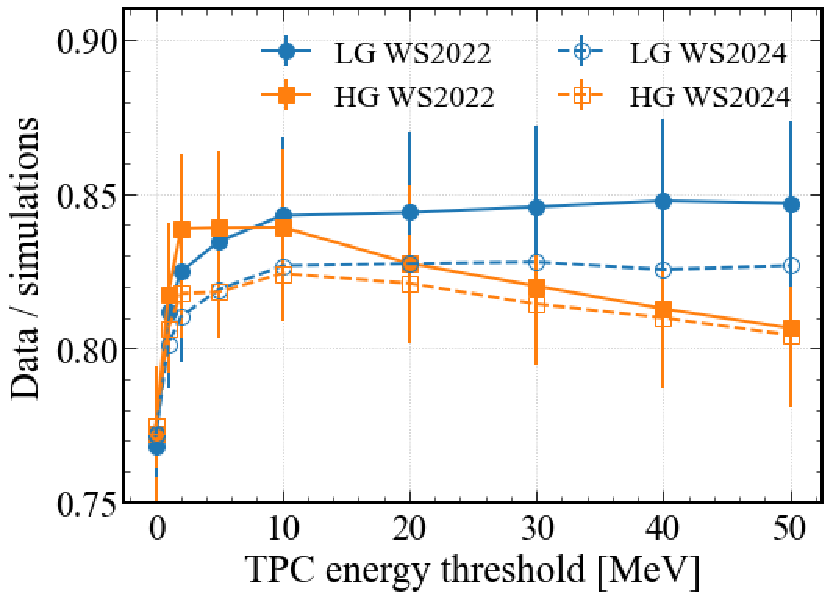
\includegraphics[width=1\textwidth,angle=0]{figures/Muons/HGLG_comp.pdf}
    \caption{}
    \label{fig:Muons/TPCHGLGComp_ratios}
    \end{subfigure}
    \caption{(a) Histograms comparing the spectrum of deposited energy in the TPC from BACCARAT muons with the spectrum of deposited energy in the TPC from WS2022 and WS2024 HG (LG) data (converted from TPC total pulse area). (b) The ratios of HG (LG) WS2022 and WS2024 data to BACCARAT simulations as a function of the energy threshold in the TPC.}
    \label{fig:Muons/TPCHGLGComp}
\end{figure}
A steady ratio of data and simulation rates was one reason we measured the flux using LG data. A low threshold such as $<~1$~MeV, would not be useful because these events are not full muon events as seen through handscanning events around this threshold. They tend to be the end of a muon cascade in both data and simulations. \autoref{fig:Muons/Muon_PID} demonstrates this by showing that most events $>~10$~MeV are muons, not muon secondaries, as it separates the events with a muon passing through the TPC from those that do not. A higher energy threshold such as $<~50$~MeV would also not be useful, as \autoref{fig:Muons/TPCHGLGComp_energy} illustrates, the effect of PMT saturation can be seen above this energy in data.
\begin{figure}[htbp]
    \centering
    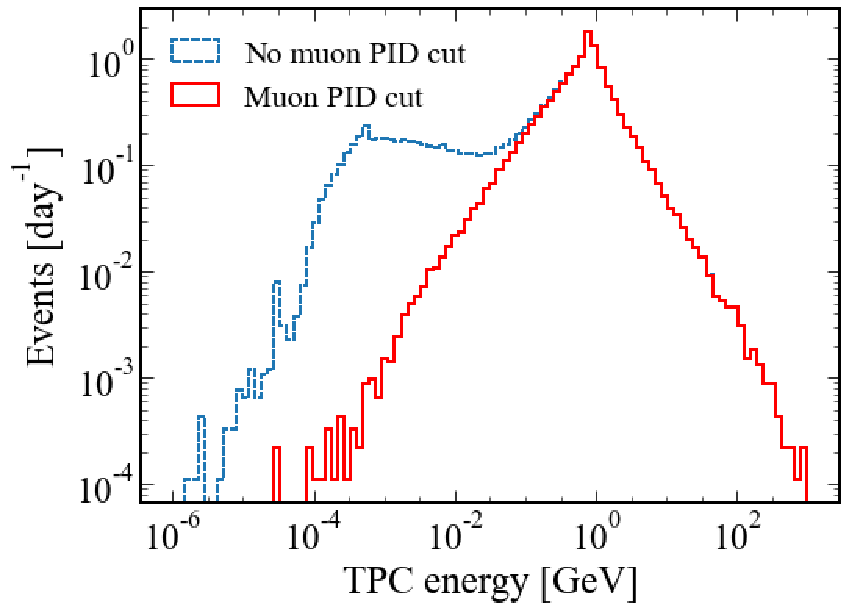
\includegraphics[width=0.65\textwidth]{figures/Muons/Muon_pid_cutLZstyle.pdf}
    \caption{Energy deposition spectra of muon events from BACCARAT simulations with and without a muon particle ID (PID) cut. The cut selects events that had a muon depositing energy in the TPC directly.}
    \label{fig:Muons/Muon_PID}
\end{figure}

\subsubsection{Lack of skin threshold}\label{sec:Muons/MuonFluxSkinThreshold}
This analysis considers a triple coincidence between the OD, Skin and TPC. However, all that is required in the Skin detector is a pulse which is classified as a `max pulse' in LZap and the pulse must have an amplitude greater than 1~phd/ns. Due to the lack of calibration and subsequent energy reconstruction in the skin, it was chosen not to set an energy threshold in the Skin as it would be difficult to make comparisons to the energy-only simulations produced using BACCARAT.

\subsection{NEST - Muon simulations and light-energy conversion}\label{sec:Muons/MuonFluxNEST}
NEST has been used to reconstruct the energy of muons traversing the TPC. Typically particle interactions are observed through an `S1' pulse and an `S2' pulse and using methods described here \cite{NEST1}, the energy deposit can be calculated. When a muon traverses the xenon space, a series of S1 and S2 pulses are produced which can not be separated in data. NEST, however, has a minimum ionising particle (MIP) module in which the linear energy transfer can be set. This is 2.1~MeV~cm$^2$~g$^{-1}$\cite{MUE} for a muon in liquid xenon with an average energy of 283~GeV. Two final inputs to NEST to simulate a muon are the start and end points of the track.\\
Sampling the start position and direction vector produced by the MUSUN simulations, all 48.2~million muons were projected down towards the LZ detector. If the muon passed through the xenon space, the point at which it entered and exited the TPC was saved and later used as the input into NEST. 67918 muons from BACCARAT passed through the xenon volume and were used towards producing the conversion between energy deposit and light produced due to the interaction. NEST outputs the energy, total S1 light and total S2 light and for the conversion used in this analysis, the S1 and S2 light was summed.
Two separate sets of conversion factors were determined through running NEST with the WS2022 LZ detector configuration and WS2024 detector configuration. An example of the comparison can be seen in \autoref{fig:Muons/nestcomparison}.
\begin{figure}[htbp]
    \centering
    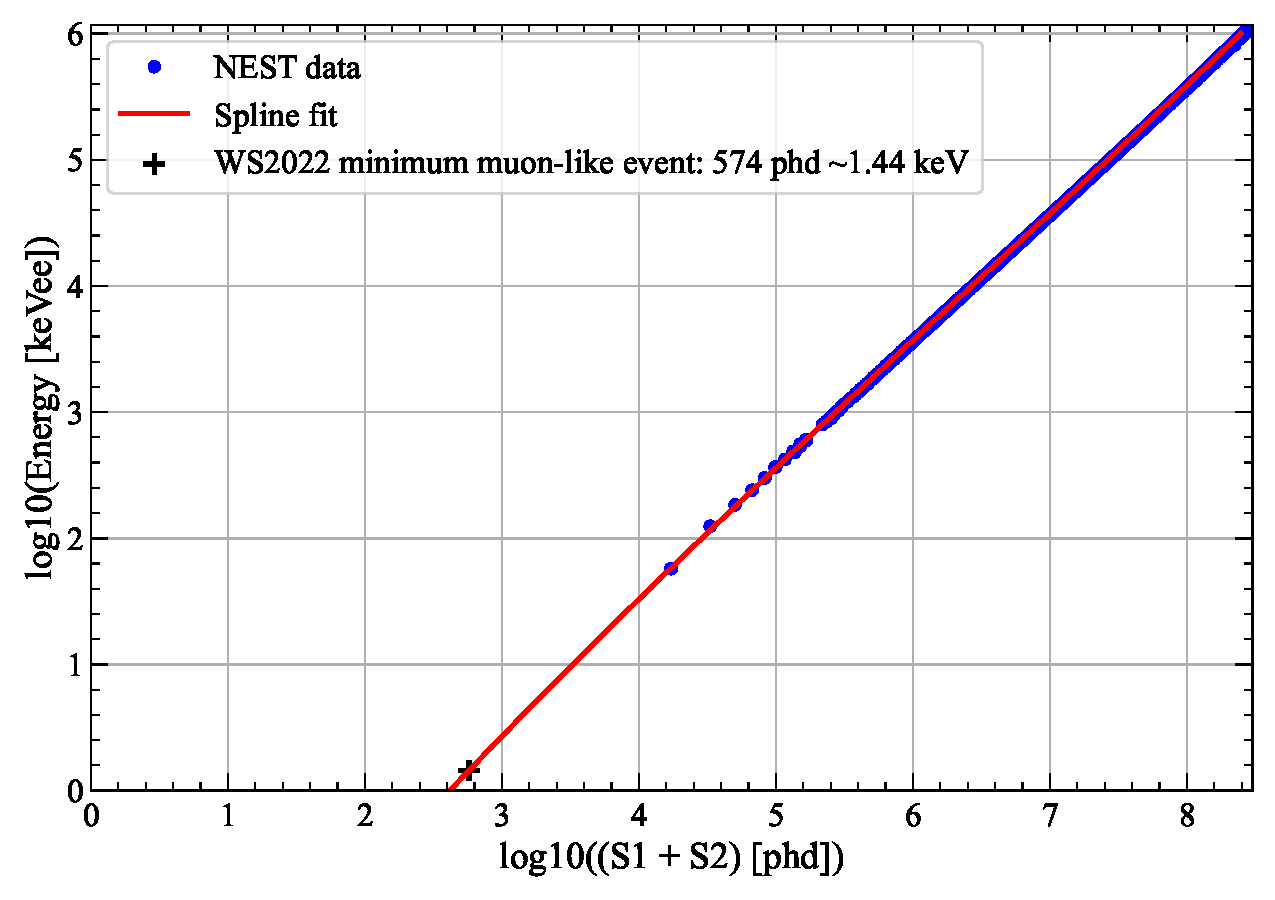
\includegraphics[width=0.8\textwidth]{figures/Muons/TPCEnergyConversion.pdf}
    \caption{Deposited energy from BACCARAT simulations versus the number of detected photons from NEST simulations. The minimum muon-like event found in data is overlaid at 574~phd and the spline fit is extrapolated down to this value.}
    %Energy to light comparison produced by simulating MIPs using NEST. The S1 and S2 light outputs have been summed together as seen in data. 
    \label{fig:Muons/nestcomparison}
\end{figure}
A spline fit was fitted to the NEST data and extrapolated down to the minimum data point at 574~phd that passed our OD energy and inter-detector timing selection. The spline fit was then used to convert the Total Pulse Area observed in a muon event window to energy. To reproduce this conversion using the following parameters in a spline fit, SciPy's {\asciifamily interpolate.BSpline}.
\begin{lstlisting}
WS2022 Parameters
t: [0.08294199 0.08294199 0.08294199 0.08294199 4.14709934 8.21125669
 8.21125669 8.21125669 8.21125669]
c: [-2.70501286 -1.03606704  1.88505502  4.49568078  5.91208229  0.
  0.          0.          0.        ]
k: 3

WS2024 Parameters
t: [0.08294199 0.08294199 0.08294199 0.08294199 4.14709934 8.21125669
 8.21125669 8.21125669 8.21125669]
c: [-2.62556966 -0.95670208  1.96474676  4.57569338  5.99200743  0.
  0.          0.          0.        ]
k: 3
\end{lstlisting}
where {\asciifamily t} is the knots, {\asciifamily c} is the spline coefficients and, {\asciifamily k} is the B-Spline degree factor.
% Prior to determining the TPC threshold, an event which passed our OD energy and inter-detector timing selection was found with a total TPC pulse area of 574~phd. 
The spline fit was extrapolated down to 574~phd to obtain a corresponding energy deposition of 1.44~keV. This energy was used as our minimum threshold when determining the TPC threshold.

\subsection{Comparison between data and simulation}\label{sec:Muons/MuonFluxDataSimComp}
LZLAMA processed the BACCARAT files to convert energy depositions into S1s, S2s and other observed quantities that we could directly compare with the WIMP Search data. However, the decision was made to only use BACCARAT simulations for two reasons: Firstly, LZLAMA is not tuned for highly ionising tracks made by muons through the TPC. The spectrum of the total pulse area in the data was very different from that which LZLAMA produced from BACCARAT, in both the TPC and OD. Conversely, the BACCARAT energy spectra in the TPC and OD had a very comparable shape to that of the data. Secondly, LZLAMA does not account for secondary particles such as pions and kaons. Initially, LZLAMA halted the processing of a file if it found an unrecognised particle ID in an event, and would move on to the next root file, which caused a great loss in the total number of events. The particle IDs for these error-triggering events were integrated into the LZLAMA source code. As a result, instead of encountering an error, a warning message was generated, quoting the particle ID, and the respective event was skipped over, thus ensuring that the remaining events in the file were not missed. A total of 767 events were missed causing slight bias since this cannot happen in data. In summary, the BACCARAT simulations were found to bear more resemblance to the spectra in data. They were also determined to have less systematic uncertainty than the LZLAMA data for processing muons and their secondary particles. Hence, we shall hereafter focus only on comparing the BACCARAT output to data.

Recording the photon production from muon interactions in the OD, skin and TPC would be too computationally intensive to use NEST as muons are highly ionising, so BACCARAT records only the energy deposited by a muon as it travels through the detector volumes. Consequently, to compare the muon flux of data and simulations, the conversion of pulse area to energy had to be determined. In previous investigations, the relationship between the photons detected by OD PMTs and the energy deposited in the OD was found to be linear at higher energies \cite{OD_linear}. On this basis, our conversion factor was estimated by superposing the two spectra and matching the broad peaks of the WS2022 and WS2024 total pulse area spectra with the broad peak of the simulated energy spectrum (in energy units). The conversion factor for both WS2022 and WS2024 is $6.5\times10^{-6}$~GeV/phd. The superposition is depicted in \autoref{fig:Muons/OD_comp} where it can be seen how closely the different features of the data spectra (summed) line up with their simulated counterparts.

The cuts introduced in the simulations were designed to mimic those applied to data, namely a coincidence cut where a muon had to pass through each of the OD, skin and TPC within an event; and the 8~MeV energy threshold, previously explained in Section 4.1. \\

\begin{figure}[htbp]
    \centering
    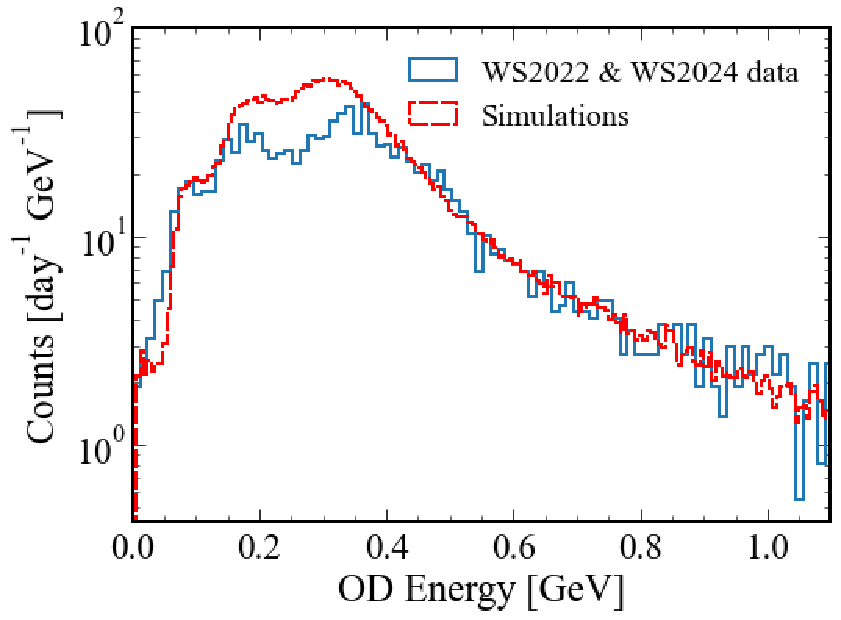
\includegraphics[width=0.65\textwidth]{figures/Muons/OD_comparison.pdf}
    %\caption{Energy deposited in the OD by muons generated by BACCARAT and the energy of events in data converted from the total pulse area in the OD.}
    \caption{Energy deposited by BACCARAT simulated muons in the OD and the energy of events in data converted from the total pulse area in the OD.}
    \label{fig:Muons/OD_comp}
\end{figure}
\par After converting both TPC and OD pulse area to energy we were able to directly compare their combined energy maps between simulated results and data. The plots displaying the full energy distributions (after coincidence and OD energy cuts) and similar distributions after the TPC 10 MeV cut is imposed are in \autoref{fig:Muons/ODTPC_comp}. Since we cannot distinguish between secondaries of muons and actual muons, we need the cut to ensure that this systematic uncertainty, which is higher at lower energies, is avoided as much as possible. The energy distributions show that the 10 MeV cut removes events with a small amount of energy deposited in the TPC and a large amount of energy deposited in the OD. This is characteristic of muon secondaries or muons that may have skimmed the edge of the TPC. 

\begin{figure}[htbp]
    \begin{subfigure}{0.49\textwidth}
    \centering
    \centering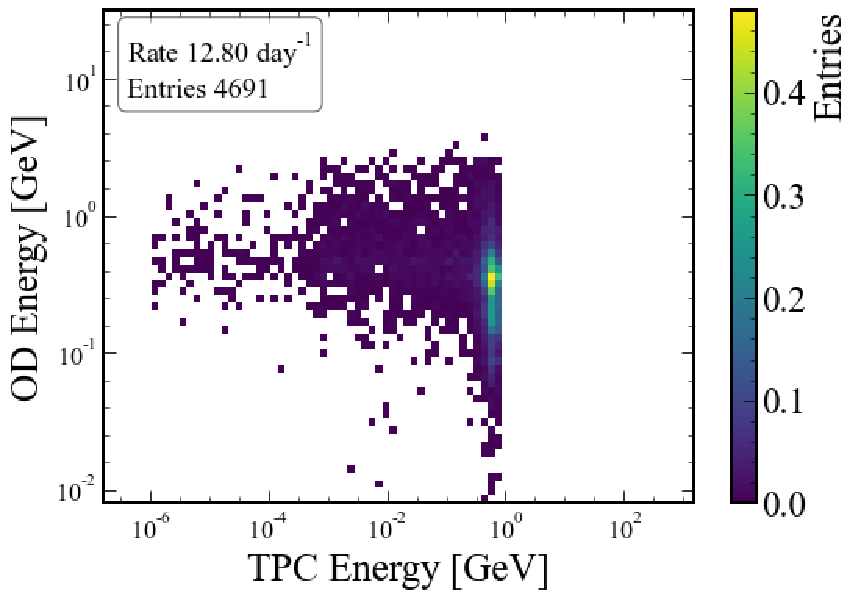
\includegraphics[width=1\textwidth,angle=0]{figures/Muons/OD_TPC_datacc.pdf}
    \caption{}
    \end{subfigure}
    \begin{subfigure}{0.49\textwidth}
    \centering
    \centering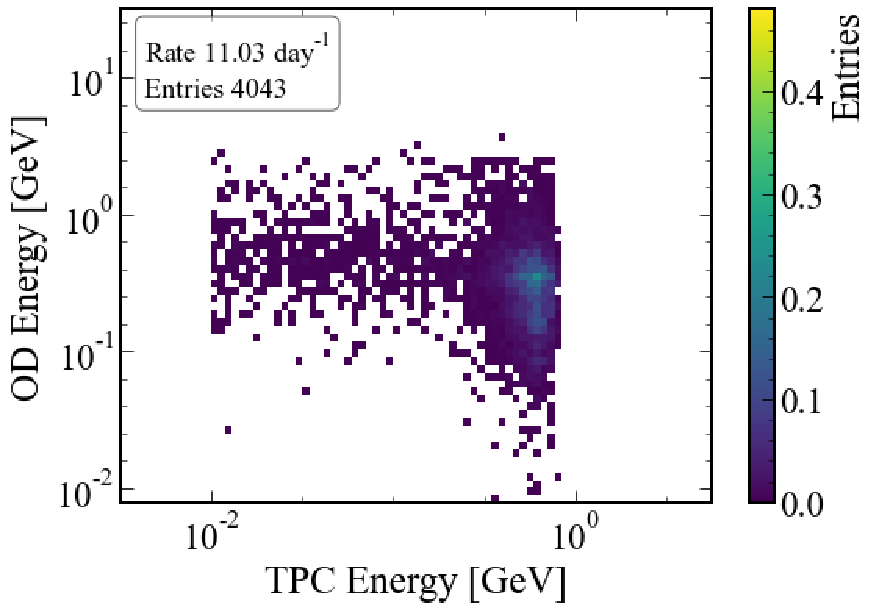
\includegraphics[width=1\textwidth,angle=0]{figures/Muons/OD_TPC_data10.pdf}
    \caption{}
    \end{subfigure}
    \begin{subfigure}{0.49\textwidth}
    \centering
    \centering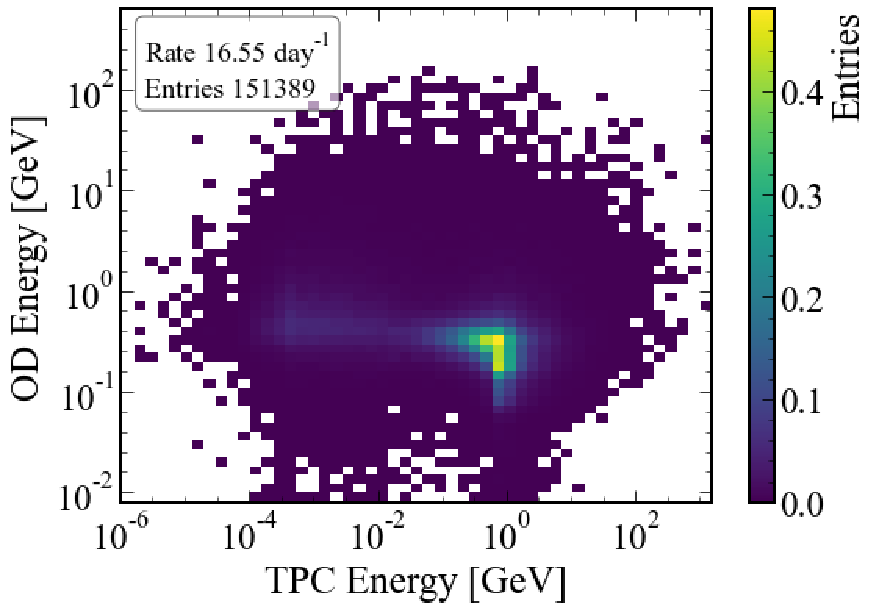
\includegraphics[width=1\textwidth,angle=0]{figures/Muons/OD_TPC_bacc0.pdf}
    \caption{}
    \end{subfigure}
    \begin{subfigure}{0.49\textwidth}
    \centering
    \centering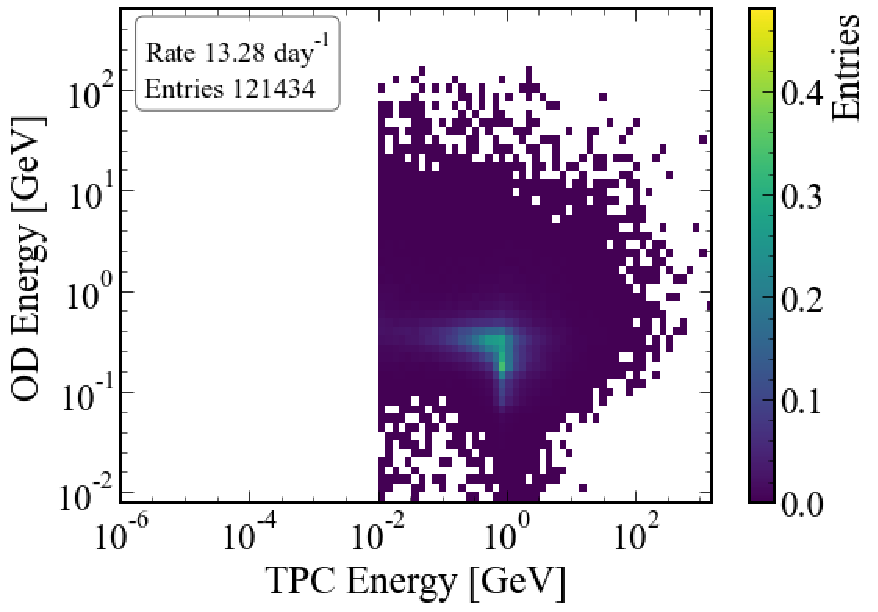
\includegraphics[width=1\textwidth,angle=0]{figures/Muons/OD_TPC_bacc10.pdf}
    \caption{}
    \end{subfigure}
    \caption{Energy depositions from events in the OD and TPC are shown, with the total pulse area from WS2022 and WS2024 data converted to energy. In (a), only OD and inter-detector timing cuts are applied, while in (b), the 10 MeV cut is also included. Similarly, BACCARAT simulations are plotted with the 8 MeV OD energy threshold and coincidence cut in (c), and with the additional 10 MeV cut included in (d).}
    \label{fig:Muons/ODTPC_comp}
\end{figure}

\subsection{Muon rate results}\label{sec:Muons/MuonRateResults}
The measured muon rates from simulations, HG and LG data for WS2022 and WS2024 are presented in, respectively, \autoref{tab:Rates2022} and \autoref{tab:Rates2024} with increasing TPC energy thresholds. By varying the TPC energy threshold (translated from total pulse area via the NEST conversion) the change in the ratio of the simulated muon rate to the muon rate from data can be tracked. Columns 4 and 6 in each table show these ratios for LG and HG data respectively, and they are also displayed in \autoref{fig:Muons/TPCHGLGComp}b. The final column in each table lists the differences between these HG and LG ratios for every threshold. As described in Section 4.3, the steadiness of the LG ratio compared to the HG ratio above 10~MeV was the major factor in our decision to implement a 10~MeV threshold and use LG data for reconstructing the muon flux (see Section 9).

\begin{center}
\begin{minipage}{\textwidth}
\def\arraystretch{1.4}%
\centering
\begin{longtable}[hbtp]{|c|c|c|c|c|c|c|}
\caption{Muon rates from simulations and WS2022 data. The data has the OD cuts and timing selections applied. The simulations have a 3-fold detector coincidence criteria and the 8~MeV OD energy cut applied. The TPC energy thresholds represent the total energy deposited by a muon event in the TPC.\newline}
\label{tab:Rates2022} \\
\hline
\multicolumn{1}{|c|}{\textbf{TPC}} & \multicolumn{1}{c|}{\textbf{Simulation}} & \multicolumn{1}{c|}{\textbf{Data LG}} & \multicolumn{1}{c|}{\textbf{Data/sims}} & \multicolumn{1}{c|}{\textbf{Data HG}} & \multicolumn{1}{c|}{\textbf{Data/sims}} & \multicolumn{1}{c|}{\textbf{LG ratio - }} \\ 
\multicolumn{1}{|c|}{\textbf{threshold}} & \multicolumn{1}{c|}{\textbf{rate [day$^{-1}$]}} & \multicolumn{1}{c|}{\textbf{rate [day$^{-1}$]}} & \multicolumn{1}{c|}{\textbf{LG ratio}} & \multicolumn{1}{c|}{\textbf{rate [day$^{-1}$]}} & \multicolumn{1}{c|}{\textbf{HG ratio}} & \multicolumn{1}{c|}{\textbf{HG ratio}} \\ \hline 
\endfirsthead \hline
\endlastfoot
%Core cuts (OD $>$ 8 MeV etc.) & 16.550 ± 0.043 & 13.205 ± 0.366 & 0.798 ± 0.022 & 13.205 ± 0.366 & 0.798 ± 0.022 & 0.000 ± 0.031 \\
TPC $>$ 1.44 keV &  16.550 ± 0.043 &  12.709 ± 0.359 & 0.768 ± 0.022  &  12.780 ± 0.360 & 0.772 ± 0.022  &    -0.004 ± 0.031 \\ \hline
TPC $>$ 1 MeV &  15.055 ± 0.041 &  12.224 ± 0.352 & 0.812 ± 0.023  &  12.305 ± 0.353 & 0.817 ± 0.024  &    -0.005 ± 0.033 \\ \hline
TPC $>$ 2 MeV &  14.477 ± 0.040 &  11.940 ± 0.348 & 0.825 ± 0.024  &  12.143 ± 0.351 & 0.839 ± 0.024  &    -0.014 ± 0.034 \\ \hline
TPC $>$ 5 MeV &  13.760 ± 0.039 &  11.485 ± 0.341 & 0.835 ± 0.025  &  11.546 ± 0.342 & 0.839 ± 0.025  &    -0.004 ± 0.035 \\ \hline
TPC $>$ 10 MeV &  13.275 ± 0.038 &  11.191 ± 0.337 & 0.843 ± 0.025  &  11.141 ± 0.336 & 0.839 ± 0.025  &     0.004 ± 0.036 \\ \hline
TPC $>$ 20 MeV &  12.840 ± 0.037 &  10.837 ± 0.331 & 0.844 ± 0.026  &  10.625 ± 0.328 & 0.827 ± 0.026  &     0.017 ± 0.036 \\ \hline
TPC $>$ 30 MeV &  12.597 ± 0.037 &  10.655 ± 0.328 & 0.846 ± 0.026  &  10.331 ± 0.323 & 0.820 ± 0.026  &     0.026 ± 0.037 \\ \hline
TPC $>$ 40 MeV &  12.413 ± 0.037 &  10.524 ± 0.326 & 0.848 ± 0.026  &  10.088 ± 0.320 & 0.813 ± 0.026  &     0.035 ± 0.037 \\ \hline
TPC $>$ 50 MeV &  12.258 ± 0.037 &  10.382 ± 0.324 & 0.847 ± 0.027  &   9.886 ± 0.316 & 0.807 ± 0.026  &     0.040 ± 0.037 \\
\hline
\end{longtable}
\end{minipage}%
\end{center}

\begin{center}
\begin{minipage}{\textwidth}
%\small
\def\arraystretch{1.4}%
\centering
\begin{longtable}[hbtp]{|c|c|c|c|c|c|c|}
\caption{Muon rates from simulations and WS2024 data. See the \autoref{tab:Rates2022} caption for descriptions of the applied cuts and energy thresholds.}
\label{tab:Rates2024} \\
\hline
\multicolumn{1}{|c|}{\textbf{TPC}} & \multicolumn{1}{c|}{\textbf{Simulation}} & \multicolumn{1}{c|}{\textbf{Data LG}} & \multicolumn{1}{c|}{\textbf{Data/sims}} & \multicolumn{1}{c|}{\textbf{Data HG}} & \multicolumn{1}{c|}{\textbf{Data/sims}} & \multicolumn{1}{c|}{\textbf{LG ratio - }} \\ 
\multicolumn{1}{|c|}{\textbf{threshold}} & \multicolumn{1}{c|}{\textbf{rate [day$^{-1}$]}} & \multicolumn{1}{c|}{\textbf{rate [day$^{-1}$]}} & \multicolumn{1}{c|}{\textbf{LG ratio}} & \multicolumn{1}{c|}{\textbf{rate [day$^{-1}$]}} & \multicolumn{1}{c|}{\textbf{HG ratio}} & \multicolumn{1}{c|}{\textbf{HG ratio}} \\ \hline 
\endfirsthead \hline
\endlastfoot
%Core cuts (OD $>$ 8 MeV etc.) & 16.550 ± 0.043 & 13.344 ± 0.223 & 0.806 ± 0.014 & 13.344 ± 0.223 & 0.806 ± 0.014 & 0.000 ± 0.019 \\
TPC $>$ 1.44 keV & 16.550 ± 0.043 & 12.769 ± 0.218 & 0.772 ± 0.013  & 12.821 ± 0.219 & 0.775 ± 0.013  &-0.003 ± 0.019 \\ \hline
TPC $>$ 1 MeV & 15.055 ± 0.041 & 12.063 ± 0.212 & 0.801 ± 0.014  & 12.137 ± 0.213 & 0.806 ± 0.014  &-0.005 ± 0.020 \\ \hline
TPC $>$ 2 MeV & 14.477 ± 0.040 & 11.730 ± 0.209 & 0.810 ± 0.015  & 11.838 ± 0.210 & 0.818 ± 0.015  &-0.007 ± 0.021 \\ \hline
TPC $>$ 5 MeV & 13.760 ± 0.039 & 11.270 ± 0.205 & 0.819 ± 0.015  & 11.259 ± 0.205 & 0.818 ± 0.015  & 0.001 ± 0.021 \\ \hline
TPC $>$ 10 MeV & 13.275 ± 0.038 & 10.975 ± 0.203 & 0.827 ± 0.015  & 10.941 ± 0.202 & 0.824 ± 0.015  & 0.003 ± 0.022 \\ \hline
TPC $>$ 20 MeV & 12.840 ± 0.037 & 10.624 ± 0.199 & 0.827 ± 0.016  & 10.542 ± 0.198 & 0.821 ± 0.016  & 0.006 ± 0.022 \\ \hline
TPC $>$ 30 MeV & 12.597 ± 0.037 & 10.430 ± 0.197 & 0.828 ± 0.016  & 10.258 ± 0.196 & 0.814 ± 0.016  & 0.014 ± 0.022 \\ \hline
TPC $>$ 40 MeV & 12.413 ± 0.037 & 10.246 ± 0.196 & 0.825 ± 0.016  & 10.052 ± 0.194 & 0.810 ± 0.016  & 0.016 ± 0.022 \\ \hline
TPC $>$ 50 MeV & 12.258 ± 0.037 & 10.134 ± 0.195 & 0.827 ± 0.016  &  9.858 ± 0.192 & 0.804 ± 0.016  & 0.023 ± 0.023 \\
\hline
\end{longtable}
\end{minipage}%
\end{center}

\begin{center}
\begin{minipage}{\textwidth}
%\small
\def\arraystretch{1.4}%
\centering
\begin{longtable}[hbtp]{|c|c|c|c|}
\caption{Muon rates from simulations, WS2022 and WS2024 data. See the \autoref{tab:Rates2022} caption for descriptions of the applied cuts and energy thresholds. \newline}
\label{tab:Rates_all}\\
\hline
\multicolumn{1}{|c|}{\textbf{TPC}} & \multicolumn{1}{c|}{\textbf{Simulation}} & \multicolumn{1}{c|}{\textbf{Data LG}} & \multicolumn{1}{c|}{\textbf{Data/sims}}  \\ 
\multicolumn{1}{|c|}{\textbf{threshold}} & \multicolumn{1}{c|}{\textbf{rate [day$^{-1}$]}} & \multicolumn{1}{c|}{\textbf{rate [day$^{-1}$]}} & \multicolumn{1}{c|}{\textbf{LG ratio}}  \\ \hline 
\endfirsthead \hline
\endlastfoot
%Core cuts (OD $>$ 8 MeV etc.) & 16.550 ± 0.043 & 13.307 ± 0.191 & 0.804 ± 0.012 & 13.307 ± 0.191 & 0.804 ± 0.012 & 0.000 ± 0.017 \\
TPC $>$ 1.44 keV & 16.550 ± 0.043 & 12.753 ± 0.187 & 0.771 ± 0.011 \\ \hline
TPC $>$ 1 MeV & 15.055 ± 0.041 & 12.106 ± 0.182 & 0.804 ± 0.012\\ \hline
TPC $>$ 2 MeV & 14.477 ± 0.040 & 11.787 ± 0.179 & 0.814 ± 0.013 \\ \hline
TPC $>$ 5 MeV & 13.760 ± 0.039 & 11.328 ± 0.176 & 0.823 ± 0.013  \\ \hline
TPC $>$ 10 MeV & 13.275 ± 0.038 & 11.033 ± 0.174 & 0.831 ± 0.013 \\ \hline
TPC $>$ 20 MeV & 12.840 ± 0.037 & 10.681 ± 0.171 & 0.832 ± 0.014  \\ \hline
TPC $>$ 30 MeV & 12.597 ± 0.037 & 10.490 ± 0.169 & 0.833 ± 0.014  \\ \hline
TPC $>$ 40 MeV & 12.413 ± 0.037 & 10.321 ± 0.168 & 0.832 ± 0.014  \\ \hline
TPC $>$ 50 MeV & 12.258 ± 0.037 & 10.201 ± 0.167 & 0.832 ± 0.014 \\
\hline
\end{longtable}
\end{minipage}%
\end{center}

\subsection{Reconstruction of the muon flux}\label{sec:Muons/MuonFluxReconstruction}
Reconstruction of the muon flux from the measured muon rate has been done simply by scaling the simulated muon flux by the same ratio as that for the measured-to-simulated rate:
\begin{equation}
    F_{m} = F_{s} \times \frac{R_m}{R_s},
\label{eq:flux}
\end{equation}
where $F_{m}$ and $F_{s}$ are the measured (reconstructed from the measured rate) and simulated muon fluxes through a surface of a sphere (unit detection efficiency at all angles), respectively, and $R_{m}$ and $R_{s}$ are the measured and simulated muon rates through the detector.

This simple scaling is based on the common inputs to the simulation of the muon flux and muon rate, namely, muon energy spectra and angular distributions at SURF. It also relies on the assumption that muon transport through the detector and detector response are correctly simulated in the LZ simulation framework BACCARAT (based on GEANT4 toolkit). Simulating muon-induced cascades and their development in and outside the detector has associated uncertainties that are difficult to estimate. By requiring the energy deposition in the TPC to be greater than 10~MeV, we effectively select events when a muon passes through the TPC and remove a relatively small contribution of events without a muon, when only low-energy secondary particles enter the TPC. No other energy cut is included so all events with a muon in the TPC (both in data and simulations) are considered in the analysis. Simulation of muon track passing through the detector and muon energy loss from ionisation along the track should be handled accurately by GEANT4. The second assumption about an accurate simulation of detector response becomes non-critical because the rate of events does not include information about energy deposition apart from the energy threshold. The ratio of measured-to-simulated rates does not depend much on the energy threshold around and above 10 MeV and the small difference in this ratio with changing the threshold can serve as an estimate of the systematic uncertainty. 

A very low energy threshold is used for the skin, only to remove noise events. Similarly, energy threshold and pulse shape analysis in the OD only remove radioactive background and noise events leaving muon events intact. Hence, we do not anticipate any uncertainty linked to the thresholds in the skin or the OD.

The ratio of measured-to-simulated muon rates for low gain in \autoref{tab:Rates_all} remains constant within statistical uncertainty for TPC energy thresholds of 5-50 MeV. For the TPC threshold of 10~MeV, this ratio is $0.831 \pm 0.013 \textrm{ (stat.)} \pm 0.008 \textrm{ (syst.)}$, where systematic uncertainty is estimated from the change in the ratio with changing the threshold by a factor of 2-3. (Note that reducing the threshold will increase the fraction of events when a muon does not enter the detector thus increasing the dependence on simulation details).

Using \autoref{eq:flux}, the ratio of $0.831 \pm 0.013 \textrm{ (stat.)} \pm 0.008 \textrm{ (syst.)}$ and the simulated muon flux of $6.16 \times10^{-9}$~cm$^{-2}$~s$^{-1}$, we derive the reconstructed muon flux from the rate measurements as $(5.119 \pm 0.080 \textrm{( stat.)} \pm 0.049 \textrm{ (syst.)})\times10^{-9}$~cm$^{-2}$~s$^{-1}$. This flux agrees well with the measurement in the nearby cavern reported in Ref.~\cite{majorana} ($(5.31 \pm 0.17)\times10^{-9}$~cm$^{-2}$~s$^{-1}$).

\subsection{Evaluation of average rock density}\label{sec:Muons/RockDensity}

The difference in the reconstructed and simulated muon fluxes is primarily due to a different density of rock compared with the initial muon model. We assume here that the surface profile is known with sufficient accuracy and so is the laboratory position. There is a small dependence of the flux on the position within the laboratory but it is below the statistical uncertainty. The dependence of the flux on the rock composition has the second-order effect. If we attribute the lower muon flux in the measurements to the higher average rock density, we can evaluate what the realistic average rock density above and around the LZ location is. 

We have calculated the muon flux at SURF with different densities of rock above the laboratory to match the measured (reconstructed from measurements) value. In this case, we used a simple approximation of a `flat' surface profile above the lab taking into account only the Earth curvature (though with negligible effect for the flux at this depth). The simulated muon flux is matched with the measured one assuming the average density of $(2.78 \pm 0.01)$~g/cm$^3$ which is 3.0\% higher than initially assumed in the muon model (see \autoref{fig:Muons/flux_density} for the flux dependence on the rock density). The statistical uncertainty of the muon rate measurements dominates the error here. This density is smaller than that reported in Ref.~\cite{majorana} ($(2.89 \pm 0.06)$~g/cm$^3$) despite almost the same muon flux. 
The muon flux has been reconstructed for the place where the measurements of the rate were carried out, namely in the Davis cavern. The flux depends on the position in and around the cavern. For example, the muon flux 7~m above the cavern from where most muons in the simulations originated will be about 3\% higher. 

%\textcolor{red}{VK: It would be good to plot the graph: muon flux vs average density of rock and indicate the measured intensity. The numbers below are for SURF rock but the result for density is practically independent of the rock composition.}
\begin{figure}[htbp]
    \centering
    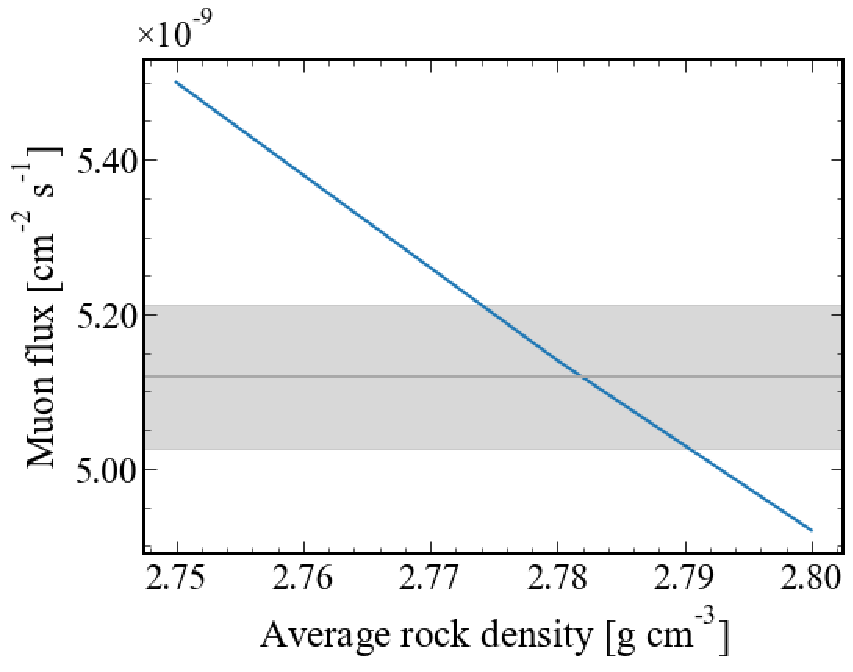
\includegraphics[width=0.65\textwidth]{figures/Muons/Flux_density_ws22_ws24.pdf}
    \caption{The muon flux dependence on average rock density within the muon model. The horizontal line and shaded section mark, respectively, the measured flux value and the combined statistical and systematic errors, $(5.119~\pm~0.094)~\times10^{-9}~\textrm{cm}^{-2}\textrm{s}^{-1}$.}
    \label{fig:Muons/flux_density}
\end{figure}


\section{Modulation}\label{sec:Muons/MuonModulation}
\subsection{Muon pulse shape in the outer detector}\label{sec:Muons/MuonModulationODPulseShape}
%\subsection{MMS analysis}

\section{Veto for WIMP search}\label{sec:Muons/MuonVeto}
Muons pose a threat to the WIMP search in multiple ways aside from the aforementioned muon induced backgrounds. As shown in \autoref{fig:Muons/eventViewer}, in the initial muon event a train of pulses characterised as \textit{S2}-like dominate the post trigger window. Depending on the energy  of the incoming muon and the length of the track which the muon takes through the xenon within the TPC, \textit{S2}-like pulses and \textit{SE}-like pulses associated with the track of ionisation can be observed for up to 2~s after the initial muon event. In addition to the train of \textit{S2}-like pulses and \textit{SE}-like pulses, \textit{SPE} pulses associated with the muon event can be observed for up to 20~s. The train of pulses following a muon event will be termed a `muon tail' in the rest of the section. During the 20~s window following a muon event the ability to differentiate a distinct single scatter produced by a WIMP from the muon tail is dramatically reduced. The `muon veto' algorithm was thus developed to remove events which contained the muon tail. An example muon tail produced from a 257~MeV energy deposition in the TPC (energy reconstructed using the spline parameters for WS2024 run in \autoref{sec:muon}).

\subsection{Cut description}\label{sec:Muons/MuonVetoCutDesc}
To identify the initial muon event, a similar selection to that used in the muon flux measurement (\autoref{sec:Muons/MuonFluxMeasurementWithLZ} was developed. The algorithm searches for an event with the following criteria:
\begin{itemize}
    \item Pulse in both the OD and Skin
    \item OD Pulse Area $>$ 2000~\unit{phd}
    \item OD PMT Coincidence $>$ 100
    \item OD Pulse Shape (Peak Amplitude/Pulse Area) $>$ 0.003~\unit{ns^{-1}}
    \item Skin Pulse Area $>$ $10^{2.75}$~\unit{phd}
    \item -100~\unit{ns} $<$ Time difference between OD and Skin Pulse $<$ 100~\unit{ns}
    \item Total TPC Pulse Area $>$ $10^{6.75}$~\unit{phd}
\end{itemize}
The time of muon events are stored within a global variable. Any event with a trigger time within 20~s from a muon event is then vetoed. For 